%%%%%%%%%%%%%%%%%%%%%%%%%%%%%%%%%%%%%%%%%
% FRI Data Science_report LaTeX Template
% Version 1.0 (28/1/2020)
% 
% Jure Demšar (jure.demsar@fri.uni-lj.si)
%
% Based on MicromouseSymp article template by:
% Mathias Legrand (legrand.mathias@gmail.com) 
% With extensive modifications by:
% Antonio Valente (antonio.luis.valente@gmail.com)
%
% License:
% CC BY-NC-SA 3.0 (http://creativecommons.org/licenses/by-nc-sa/3.0/)
%
%%%%%%%%%%%%%%%%%%%%%%%%%%%%%%%%%%%%%%%%%


%----------------------------------------------------------------------------------------
%	PACKAGES AND OTHER DOCUMENT CONFIGURATIONS
%----------------------------------------------------------------------------------------
\documentclass[fleqn,moreauthors,10pt]{ds_report}
\usepackage[english]{babel}
\usepackage{csquotes}
\usepackage{tcolorbox}
\usepackage{calc}
\usepackage{booktabs}

\usepackage{enumitem}
\setitemize{noitemsep,topsep=0pt,parsep=0pt,partopsep=0pt}


\newsavebox\mybox
\newenvironment{aquote}[1]
  {\savebox\mybox{#1}\begin{quote}\openautoquote\hspace*{-.7ex}}
  {\unskip\closeautoquote\vspace*{1mm}\signed{\usebox\mybox}\end{quote}}

\graphicspath{{fig/}}


\newtcbox{\labelbox}[1][red]{on line,
arc=0pt,outer arc=0pt,colback=#1!10!white,colframe=#1!50!black,
boxsep=0pt,left=1pt,right=1pt,top=1pt,bottom=0.8pt,
boxrule=0pt,bottomrule=0.6pt,toprule=0.6pt,width=5cm}

\newcommand\bm{0.2pt}


%----------------------------------------------------------------------------------------
%	ARTICLE INFORMATION
%----------------------------------------------------------------------------------------

% Header
\JournalInfo{FRI Natural language processing course 2021}

% Interim or final report
\Archive{Project report} 
%\Archive{Final report} 

% Article title
\PaperTitle{Offensive language exploratory analysis} 

% Authors (student competitors) and their info
\Authors{Maša Kljun, Matija Teršek}

% Advisors
\affiliation{\textit{Advisors: Assist. Prof. dr. Slavko Žitnik}}

% Keywords
\Keywords{Offensive language, hate speech, natural language processing, traditional methods, contextual and non-contextual embeddings, exploratory analysis, ...}
\newcommand{\keywordname}{Keywords}


%----------------------------------------------------------------------------------------
%	ABSTRACT
%----------------------------------------------------------------------------------------

\Abstract{
In this paper we focus on the exploratory analysis of 21 different subgroups of offensive language. We use natural language processing techniques in order to find the underlying structure and connections/relations between the subgroups. We focus on data extracted from Twitter and online forums from 7 different data sets. First, we use classic approaches, such as TF–IDF, BoW, and LDA, then we move on to more sophisticated embeddings. We use both, non-contextual embeddings, such as Word2Vec, GloVe, and FastText, and contextual embeddings, such as BERT, KeyBERT, and USE. We find out that all subgroups are tightly connected in the sense of contextual embeddings. Considering all results, we provide a possible ontology of offensive language.}

%----------------------------------------------------------------------------------------

\begin{document}

% Makes all text pages the same height
\flushbottom 

% Print the title and abstract box
\maketitle 

% Removes page numbering from the first page
\thispagestyle{empty} 

%----------------------------------------------------------------------------------------
%	ARTICLE CONTENTS
%----------------------------------------------------------------------------------------

\section{Introduction}
In the last few years social media grew exponentially and with it also the ability of people to express themselves online. Enabling people to write on different online platforms without even identifying themselves lead to a new era of freedom of speech. Despite this new medium for communication bringing many positive things, it also has its downside. Social media has become a place where heated discussions happen and often result in insults and hatred. It is an important task to recognize hate speech and offensive language, and to prevent it.

Hate speech is defined as \textit{abusive or threatening speech or writing that expresses prejudice against a particular group, especially on the basis of race, religion, or sexual orientation}\cite{hate_speech}. We can see that the definition is very vague. Having said that, the goal of our paper is to help distinguish different types of hate speech and find the specific keywords of its subgroups in order to explain its structure. This could help with its identification and classification. In this paper we focus on 21 subgroups of offensive language - \textit{abusive, hateful, spam, general hate speech, profane, offensive, cyberbullying, racism, sexism, vulgar, homophobic, slur, harassment, obscene, threat, discredit, insult, hostile, toxic, identity hate} and \textit{benevolent sexism}. The goal of this paper is to explore offensive language subgroups and understand the similarities and connections between them. 

There has been done a lot of research regarding the offensive language, however, these works are usually focused on the classification. One of the first works include \cite{spertus1997smokey} who built the decision tree based classifier Smokey for abusive message recognition and classification. Some other works that focus mainly on classification include \cite{waseem2016you}, who compare the classification accuracy of models trained on expert and amateur annotations, \cite{gamback2017using} use convolutional neural networks for classification into four predefined categories, and \cite{martins2018hate} use different natural language processing techniques for expanding data sets with emotional information for better classification. In the last years, especially deep learning models are often used for detection and classification of hate speech, such as \cite{rizoiu2019transfer}, who propose a sophisticated method that is a combination of a deep neural network architecture with transfer learning.
There is also a lot of related work that focuses on creating large data sets, such as \cite{chung2019conan}, who create a large-scale, multilingual, expert based data set of hate speech. 

What is less common in the research area of offensive language is analysis of relationships between different types of offensive language and the importance of specific keywords. Some examples include \cite{xu2012learning}, who try to separate bullying from other social media posts and try to discover topic of bullying using topic modeling with Latent Dirichlet Allocation (LDA). \cite{calderon2020topic} model hate speech against immigrants on Twitter in Spain. They try to find underlying topic of hate speech using LDA, discovering features of different dimensions of hate speech, including foul language, humiliation, irony, etc. \cite{schmidt2017survey} conduct a survey about hate speech detection and describe key areas that have been explored, regarding the topic modeling, as well as sentiment analysis.

We organize this paper as follows: we present the data sets and describe data preprocessing in Section \ref{sec:data}, we perform the exploratory analysis by using many traditional and neural approaches in Section \ref{sec:metho}, and provide a possible offensive language ontology in Section \ref{sec:schema}.
% --------------------------------------------------------------------------------------------------------------------------------

\section{Data}
\label{sec:data}


\subsection{Data sets and label distribution}
We use $7$ publicly available data sets for our exploratory analysis. We combine data sets \cite{waseem2016you}, \cite{waseem2016hateful}, and \cite{jha2017does} into one large data set (referred to as SRB) as they include same categories of hate speech. We make labels \textit{sexism}, \textit{racism}, and \textit{both} from \cite{waseem2016you} and \cite{waseem2016hateful}. The third data set \cite{jha2017does} that we use contains label \textit{hostile sexism}, where marked tweets are already included in the first two data sets under \textit{sexism}, and label \textit{benevolent sexism}, which we rename to \textit{benevolent}. We obtain a data set with $6069$ samples that are labeled either $sexism$, $racism$, $both$, or $benevolent$.
The fourth data set (referred to as AHS)\cite{founta2018large} that we use has $3$ categories - \textit{abusive,
hateful, spam}. As this is the original data set, no additional merging is needed. We obtain a data set with $13776$ tweets with the mentioned labels. Note that we exclude \textit{None} label from both data sets, as we do not need it for the analysis.
We show the distribution of individual categories from data sets SRB and AHS in Figures \ref{fig:distribution_tweets_dataset1} and \ref{fig:distribution_tweets_dataset2}, respectively. Note that the numbers of samples might not match the numbers in the original papers, due to the Twitter removing the tweets, making them unavailable for us to analyze. We also provide an example for each label.

\begin{tcolorbox}[colback=black!8,width=0.9\linewidth, center,arc=8pt,sharp corners=downhill, boxrule=0.3pt, left=\bm, top=\bm, right=\bm, bottom=\bm, fontupper=\small]
\labelbox{\textit{Racism}} - "He can't be a server at our restaurant, that beard makes him look like a terrorist." Everyone laughs. \#fuckthanksgiving
\end{tcolorbox}

\begin{tcolorbox}[colback=black!8, width=0.9\linewidth, center,arc=8pt,sharp corners=downhill, boxrule=0.3pt, left=\bm, top=\bm, right=\bm, bottom=\bm, fontupper=\small]
\labelbox{\textit{Sexism}} - \#katieandnikki stop calling yourselves pretty and hot..you're not and saying it a million times doesn't make you either...STFU
\end{tcolorbox}

\begin{tcolorbox}[colback=black!8, width=0.9\linewidth, center,arc=8pt,sharp corners=downhill, boxrule=0.3pt, left=\bm, top=\bm, right=\bm, bottom=\bm, fontupper=\small]
\labelbox{\textit{Benevolent}} - It's "NEXT to every successful man, there's a woman"
\end{tcolorbox}

\begin{tcolorbox}[width=0.9\linewidth, center,arc=8pt,sharp corners=downhill, boxrule=0.3pt, left=\bm, top=\bm, right=\bm, bottom=\bm, fontupper=\small]
\labelbox{\textit{Spam}} - RT @OnlyLookAtMino: [!!] \#WINNER trending \#1 on melon search
\end{tcolorbox}

\begin{tcolorbox}[width=0.9\linewidth, center,arc=8pt,sharp corners=downhill, boxrule=0.3pt, left=\bm, top=\bm, right=\bm, bottom=\bm, fontupper=\small]
\labelbox{\textit{Abusive}} - You Worried About Somebody Bein Ugly... Bitch You Ugly...
\end{tcolorbox}

\begin{tcolorbox}[width=0.9\linewidth, center,arc=8pt,sharp corners=downhill, boxrule=0.3pt, left=\bm, top=\bm, right=\bm, bottom=\bm, fontupper=\small]
\labelbox{\textit{Hateful}} - i hope leaders just kick retards that fake leave teams today
\end{tcolorbox}

\begin{figure}[ht]\centering
	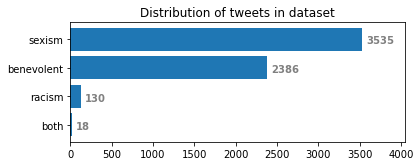
\includegraphics[width=\linewidth]{distribution_tweets_dataset1.png}
	\caption{\textbf{Distribution of tweets in SRB data set.} This figure shows the distribution of hate speech categories in the SRB data set. We can see that \textit{sexism} and \textit{benevolent} are well represented, whereas \textit{racism} and \textit{both} are far less frequent. Original set contains more tweets labeled \textit{racism}, but due to their removal we cannot obtain them.}
	\label{fig:distribution_tweets_dataset1}
\end{figure}

\begin{figure}[ht]\centering
	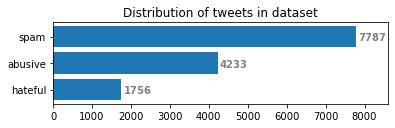
\includegraphics[width=\linewidth]{distribution_tweets_dataset2.png}
	\caption{\textbf{Distribution of tweets in AHS data set.} We see that the \textit{spam} is the most represented label in the data set, which represents the majority of the data set. This is followed by the \textit{abusive} tweets and there is the least of \textit{hateful} tweets. We can see that categories in this data set are well represented.}
	\label{fig:distribution_tweets_dataset2}
\end{figure}

\noindent Additionally, we use the data set of comments extracted from the League of Legends community \cite{bretschneider2016detecting}. We preprocess the data set given in the SQL format to a more readable CSV form and keep only the posts that are annotated as harassment. We obtain $259$ examples of cyberbullying. The sixth data set that we use was designed for the problem of the hate speech identification and classification, but we use the labels from the train and test set and merge them into one big data set that we use for our analysis. It provides tags of \textit{hatespeech, profane}, and \textit{offensive}, so we refer to the data set as HPO. It consists of 2549 tweets, distribution of which can be seen in Figure \ref{fig:distribution_tweets_hpo}. We again provide an example for each of the labels.

\begin{tcolorbox}[colback=black!8, width=0.9\linewidth, center,arc=8pt,sharp corners=downhill, boxrule=0.3pt, left=\bm, top=\bm, right=\bm, bottom=\bm, fontupper=\small]
\labelbox{\textit{Cyberbullying}} - plot twist she's a fggt
\end{tcolorbox}

\begin{tcolorbox}[width=0.9\linewidth, center,arc=8pt,sharp corners=downhill, boxrule=0.3pt, left=\bm, top=\bm, right=\bm, bottom=\bm, fontupper=\small]
\labelbox{\textit{Hatespeech}} - Johnson you liar. You don't give a flying one for the Irish
\end{tcolorbox}

\begin{tcolorbox}[width=0.9\linewidth, center,arc=8pt,sharp corners=downhill, boxrule=0.3pt, left=\bm, top=\bm, right=\bm, bottom=\bm, fontupper=\small]
\labelbox{\textit{Offensive}} - \#FuckTrump And retired porn star Melania too.
\end{tcolorbox}

\begin{tcolorbox}[width=0.9\linewidth, center,arc=8pt,sharp corners=downhill, boxrule=0.3pt, left=\bm, top=\bm, right=\bm, bottom=\bm, fontupper=\small]
\labelbox{\textit{Profane}} - Fuck Trump and anybody who voted for that Lyin POS!  \#FuckTrump
\end{tcolorbox}

\begin{figure}[ht]\centering
	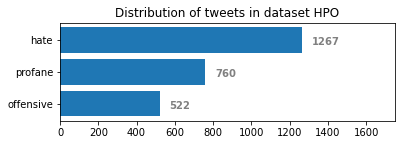
\includegraphics[width=\linewidth]{distribution_tweets_hpo.png}
	\caption{\textbf{Distribution of tweets in HPO data set.} The most used label is \textit{hatespeech}. It is followed by \textit{profane} and then \textit{offensive}, which have a similar number of tweets.}
	\label{fig:distribution_tweets_hpo}
\end{figure}

\noindent We also use the data set of Wikipedia comments \cite{dixon2017ex} that are marked as either \textit{toxic}, \textit{severe toxic}, \textit{obscene}, \textit{identity hate}, \textit{threat}, and \textit{insult}. We merge the first two categories into \textit{toxic}. It is important to note that each comment in this data set might have multiple labels, so the results for those tags might be similar. Original data set contains $159571$ tweets, $16225$ of which are labeled. We show the distribution of the labels in Figure \ref{fig:distribution_wiki_dataset}. We denote this data set as TOITI in the future text.

\begin{tcolorbox}[width=0.9\linewidth, center,arc=8pt,sharp corners=downhill, boxrule=0.3pt, left=\bm, top=\bm, right=\bm, bottom=\bm, fontupper=\small]
\labelbox{\textit{Threat}} - SHUT UP, YOU FAT POOP, OR I WILL KICK YOUR ASS!!!
\end{tcolorbox}

\begin{tcolorbox}[width=0.9\linewidth, center,arc=8pt,sharp corners=downhill, boxrule=0.3pt, left=\bm, top=\bm, right=\bm, bottom=\bm, fontupper=\small]
\labelbox{\textit{Obscene}} - you are a stupid fuck and your mother's cunt stinks
\end{tcolorbox}

\begin{tcolorbox}[width=0.9\linewidth, center,arc=8pt,sharp corners=downhill, boxrule=0.3pt, left=\bm, top=\bm, right=\bm, bottom=\bm, fontupper=\small]
\labelbox{\textit{Insult}} - Fuck you, block me, you faggot pussy!
\end{tcolorbox}

\begin{tcolorbox}[width=0.9\linewidth, center,arc=8pt,sharp corners=downhill, boxrule=0.3pt, left=\bm, top=\bm, right=\bm, bottom=\bm, fontupper=\small]
\labelbox{\textit{Toxic}} - What a motherfucking piece of crap those fuckheads for blocking us!
\end{tcolorbox}

\begin{tcolorbox}[width=0.9\linewidth, center,arc=8pt,sharp corners=downhill, boxrule=0.3pt, left=\bm, top=\bm, right=\bm, bottom=\bm, fontupper=\small]
\labelbox{\textit{Identity}} - A pair of jew-hating weiner nazi schmucks.
\end{tcolorbox}


\begin{figure}
	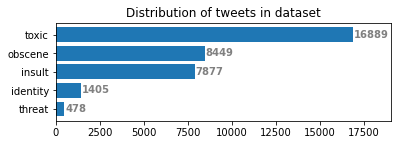
\includegraphics[width=\linewidth]{distribution_wiki_dataset.png}
	\caption{\textbf{Distribution of tweets in TOITI}. We see that most of the comments are labeled as \textit{toxic}. Around half of them are \textit{obscene} and around half are also labeled as \textit{insult}. \textit{Identity hate} and \textit{threat} are far less common in this data set.}
	\label{fig:distribution_wiki_dataset}
\end{figure}


\subsection{Annotation process of the data}
As the goal of this report is to inspect deeper structure and gain a new understanding of relationships between different subgroups of hate speech, we must also inspect how the data, that we work with, was annotated. Annotations play a big role in this analysis, as we take them as a ground truth, meaning if in the data set some tweet / comment was labeled as e.g., \textit{sexism} we do not further question this choice, and perform all our further analysis accordingly.

Data set \cite{waseem2016you} uses both amateur annotators from crowdsourcing platform CrowdFlower and annotators with theoretical and applied knowledge of hate speech, and use the data set for hate speech detection and classification. \cite{jha2017does} manually annotate their data set with the help of a 25 year old woman studying gender studies and use the data to investigate how different is benevolent sexism from sexism, and also perform classification with SVM. \cite{founta2018large} again use amateur annotators from CrowdFlower and want to provide large annotated data set that is available for further scientific exploration. \cite{bretschneider2016detecting} use 3 human experts for the annotation and then propose an approach to precisely detect cyberbullies and also provide metrics to identify victims of severe cyberbullying cases. \cite{mandl2019overview} used junior experts for language and they engaged with an online system to judge the tweets. Their goal was text classification. \cite{dixon2017ex} again use platform CrowdFlower, however, they require their annotators to first pass a test of 10 questions to ensure data quality. Their goal is to provide methodology that will allow them explore some of the open questions about the nature of online personal attacks.

\subsection{Preprocessing}
Before applying any methods we first preprocess all of our data. We remove retweet text RT, hyperlinks, hashtags, taggings, new lines, and zero length tweets. We further filter out tokens that do not contain letters, e.g., raw punctuation.

% --------------------------------------------------------------------------------------------------------------------------------
\section{Methodology}
\label{sec:metho}

\subsection{Traditional approaches}
We start the analysis with more traditional approaches, and continue with neural approaches.

% --------------------------------------------------------------

\subsubsection{LDA}
We use Latent Dirchilet Allocation (LDA) in combination with Bag-of-Words (BoW) and TF--IDF in hopes of finding obvious topics from all the provided comments / tweets. We try to determine 15 different topics, which is the same as the number of labels we have in our data sets. Results using BoW and TF--IDF are similar, however, we cannot clearly distinguish between the topics and connect obtained topics to the existing labels, aside from one topic, which is related to sexism. Top 5 most related words are: \textit{penis, rape, image, live, vagina}.

% --------------------------------------------------------------
\subsubsection{TF-IDF}
We continue with the analysis of data sets with a traditional method TF--IDF as we want to see the most relevant words for each category of offensive language that we have in the data set. We show the results in Table \ref{tab:tf-idf}. We can see that some of the categories have similar unigrams that achieved the highest TF--IDF score. An example of categories with the same highest scored unigrams are \textit{insult} and \textit{obscene}. This makes it harder to differentiate between the categories. It is important to note, that such examples might also occur due to subjective labeling in the provided data sets, as well as people not clearly differentiating between these categories. Most data sets are not labeled by experts, but with the help of platforms such as FigureEight or Amazon Mechanical Turk. From the results in Table \ref{tab:tf-idf}, we could assume that most people perceive categories such as \textit{insult} and \textit{obscene} or \textit{threat} and \textit{toxic} similarly. On the other hand, categories such as \textit{spam} or \textit{cyberbullying} are clearly differentiable from other categories. We can also see a lot of categories including Trump related words (\textit{hatespeech, profane}, and \textit{offensive}). Those categories are taken from the same data set, and we can see that such labels will contain words that are related. So the words connected to those labels might also be connected to some bigger topic, which depends on the annotator's choice from where to extract the tweets / comments.

\begin{table}[htb]
\scriptsize
\centering
\begin{tabular}{l|l}
\toprule
\textbf{category}   & \textbf{unigrams with highest TF--IDF score} \\ \midrule
racism     & peopl, white, terror, man, look                \\ \hline
sexism     & feminazi, women, think, sexist, notsexist                \\ \hline
benevolent & women, classi, sassi, nasti, gonna            \\ \hline
abusive    & know, stupid, shit, like, idiot  \\ \hline
hateful    & peopl, trump, nigga, like, idiot    \\ \hline
spam       & giveaway, game, enter, work, home            \\ \hline
cyberbullying       & one, guy, good, gone, go             \\ \hline
hatespeech      & world, trumpisatraitor, trump, shameonicc, peopl             \\ \hline
identity hate       & fuck, shit, littl, like, one             \\ \hline
insult       & delet, go, ass, stupid, bitch        \\ \hline
obscene       & delet, go, stupid, bitch, ass             \\ \hline
offensive       & trumpisatraitor, like, douchebag, fucktrump, get            \\ \hline
profane       & trump, shit, say, resist, peopl             \\ \hline
threat       & fuck, get, die, want, find           \\ \hline
toxic       & fuck, get, bitch, want, block             \\ \bottomrule
\end{tabular}
\caption{Table shows 5 highest scoring unigrams for each label we investigate. We choose the parameters, which we believe provide us the most meaningful unigrams, so we consider words that appear in at least $5\%$ and less than $60\%$ of the documents.}
\label{tab:tf-idf}
\end{table}

% --------------------------------------------------------------
\subsection{Non-contextual word embeddings}
For each of the category labels we try to find the $30$ most similar words and use their embeddings to infer the similarities and differences between the subgroups. For this task we use pre-fitted Word2Vec (\cite{mikolov2013efficient}, \cite{mikolov2013distributed}), GloVe \cite{pennington2014glove}, and FastText (\cite{bojanowski2016enriching}). We visualize the results with the help of t-SNE. Because of this we cannot interpret distances between the labels from the visualization. However, we can still infer that the labels that are intertwined are more similar than those that are nicely separable from one another. %We show the results in \ref{fig:embedding_words}. From both plots we can see that words (and its neighbors) like bitch, ass, nigga, shit, fuck, idiot, stupid, and docuhebag are relatively closely together. This could indicate a relation between \textit{abusive, hateful, insult, obscene, identity hate}, and \textit{toxic}. We can also see that classy, nasty, sassy, feminazi, and sexist are closely related - sometimes some words are more related in Word2Vec than in Glove and vice versa. From this we can see a relation between \textit{sexism} and \textit{benevolent sexism}, which is expected as they are correlated. Relationships between certain words can also vastly differ in Word2Vec and Glove. For example giveaway and game are relatively close in Word2Vec, but are further apart in Glove. Similarly, terror and white (both common unigrams of \textit{racism} label) are far away in Word2Vec, but close in Glove. However, terror stands out from other words in both embeddings, which might indicate that racism is at least in some way different to other labels. Similarly, words from \textit{spam} are usually more separated from words of other labels, also indicating another more clearly distinguishable group. Trump is relatively close to a lot of words in Word2Vec - women, world, peopl, sexist, die, little, guy. This could imply that general \textit{hatespeech} and \textit{hateful} are connected to \textit{sexism, identity hate, threat} and also \textit{cyberbullying}. 

%\begin{figure*}[htb]\centering
%	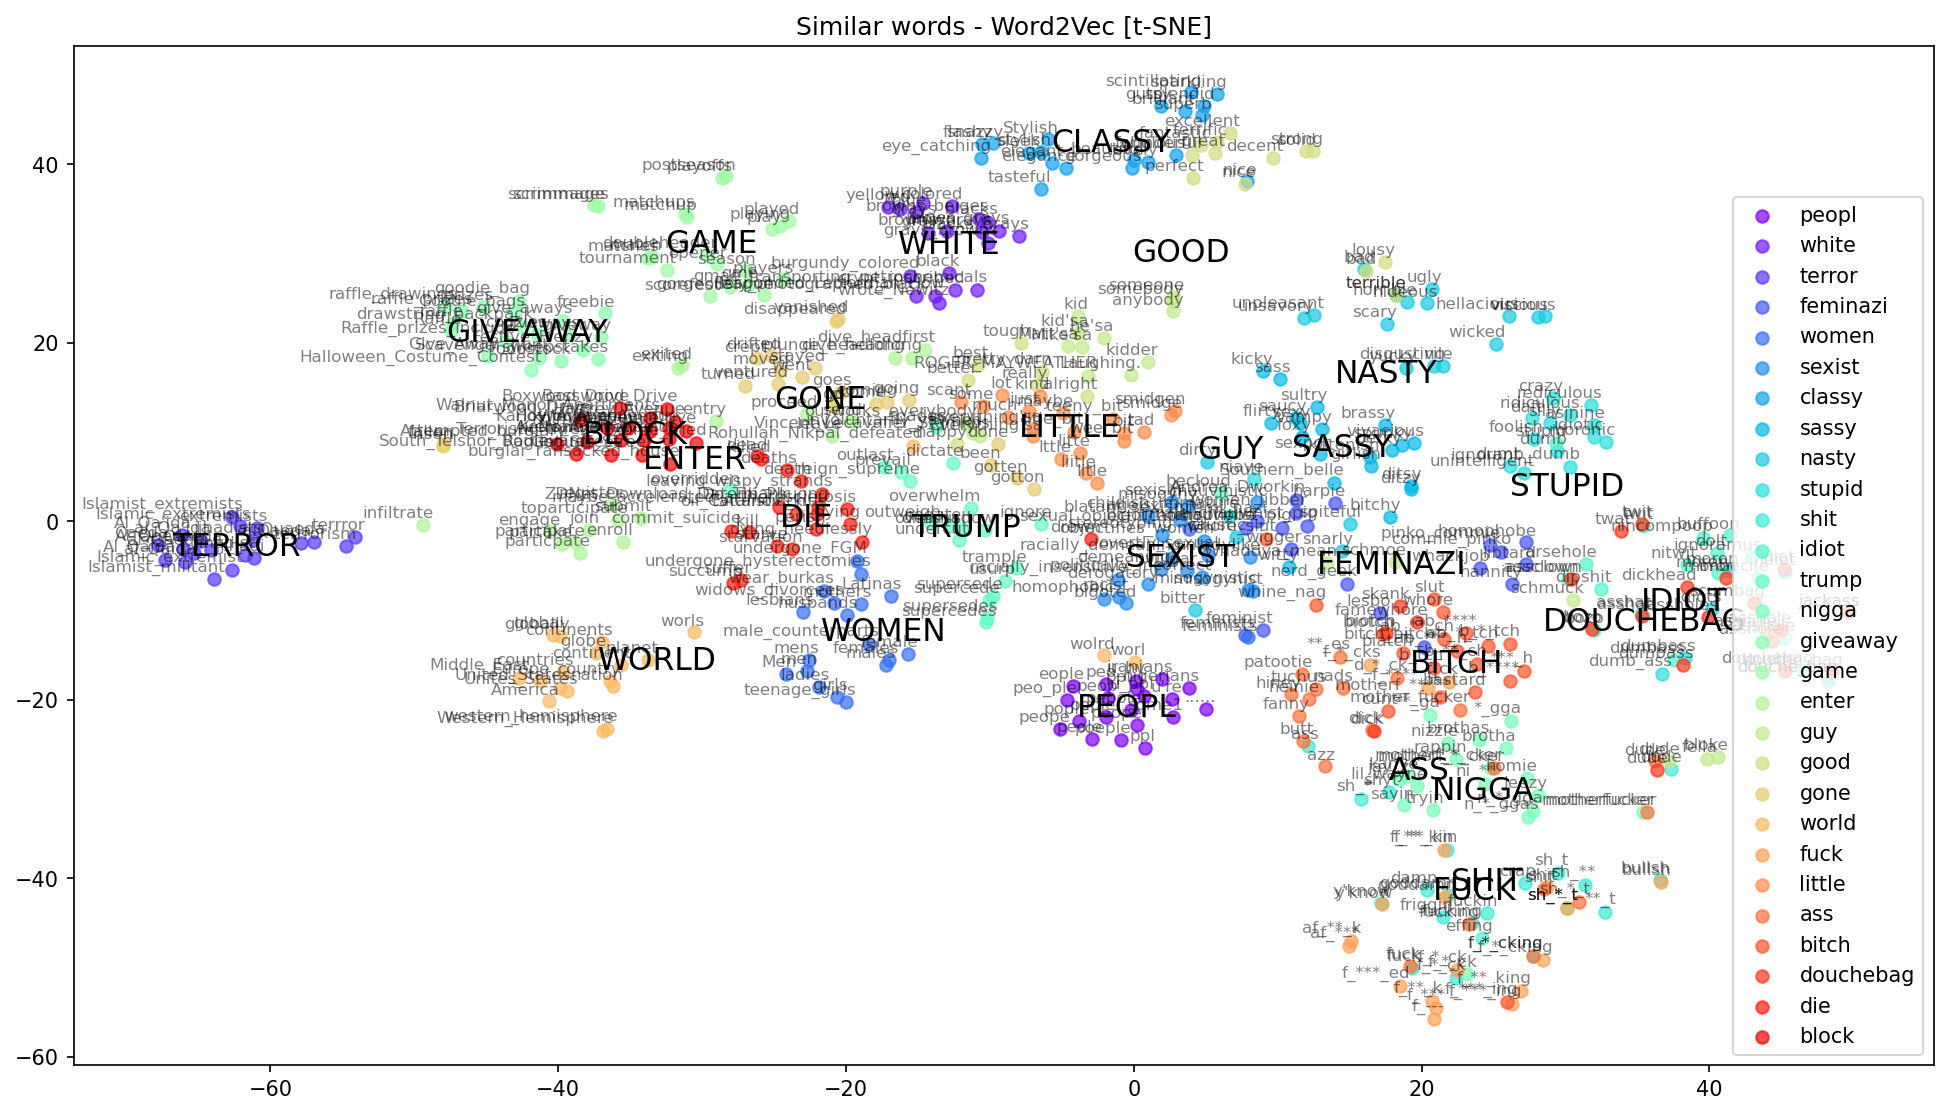
\includegraphics[width=0.495\linewidth]{SimilarWords - word2vec - t-SNE.png}
%	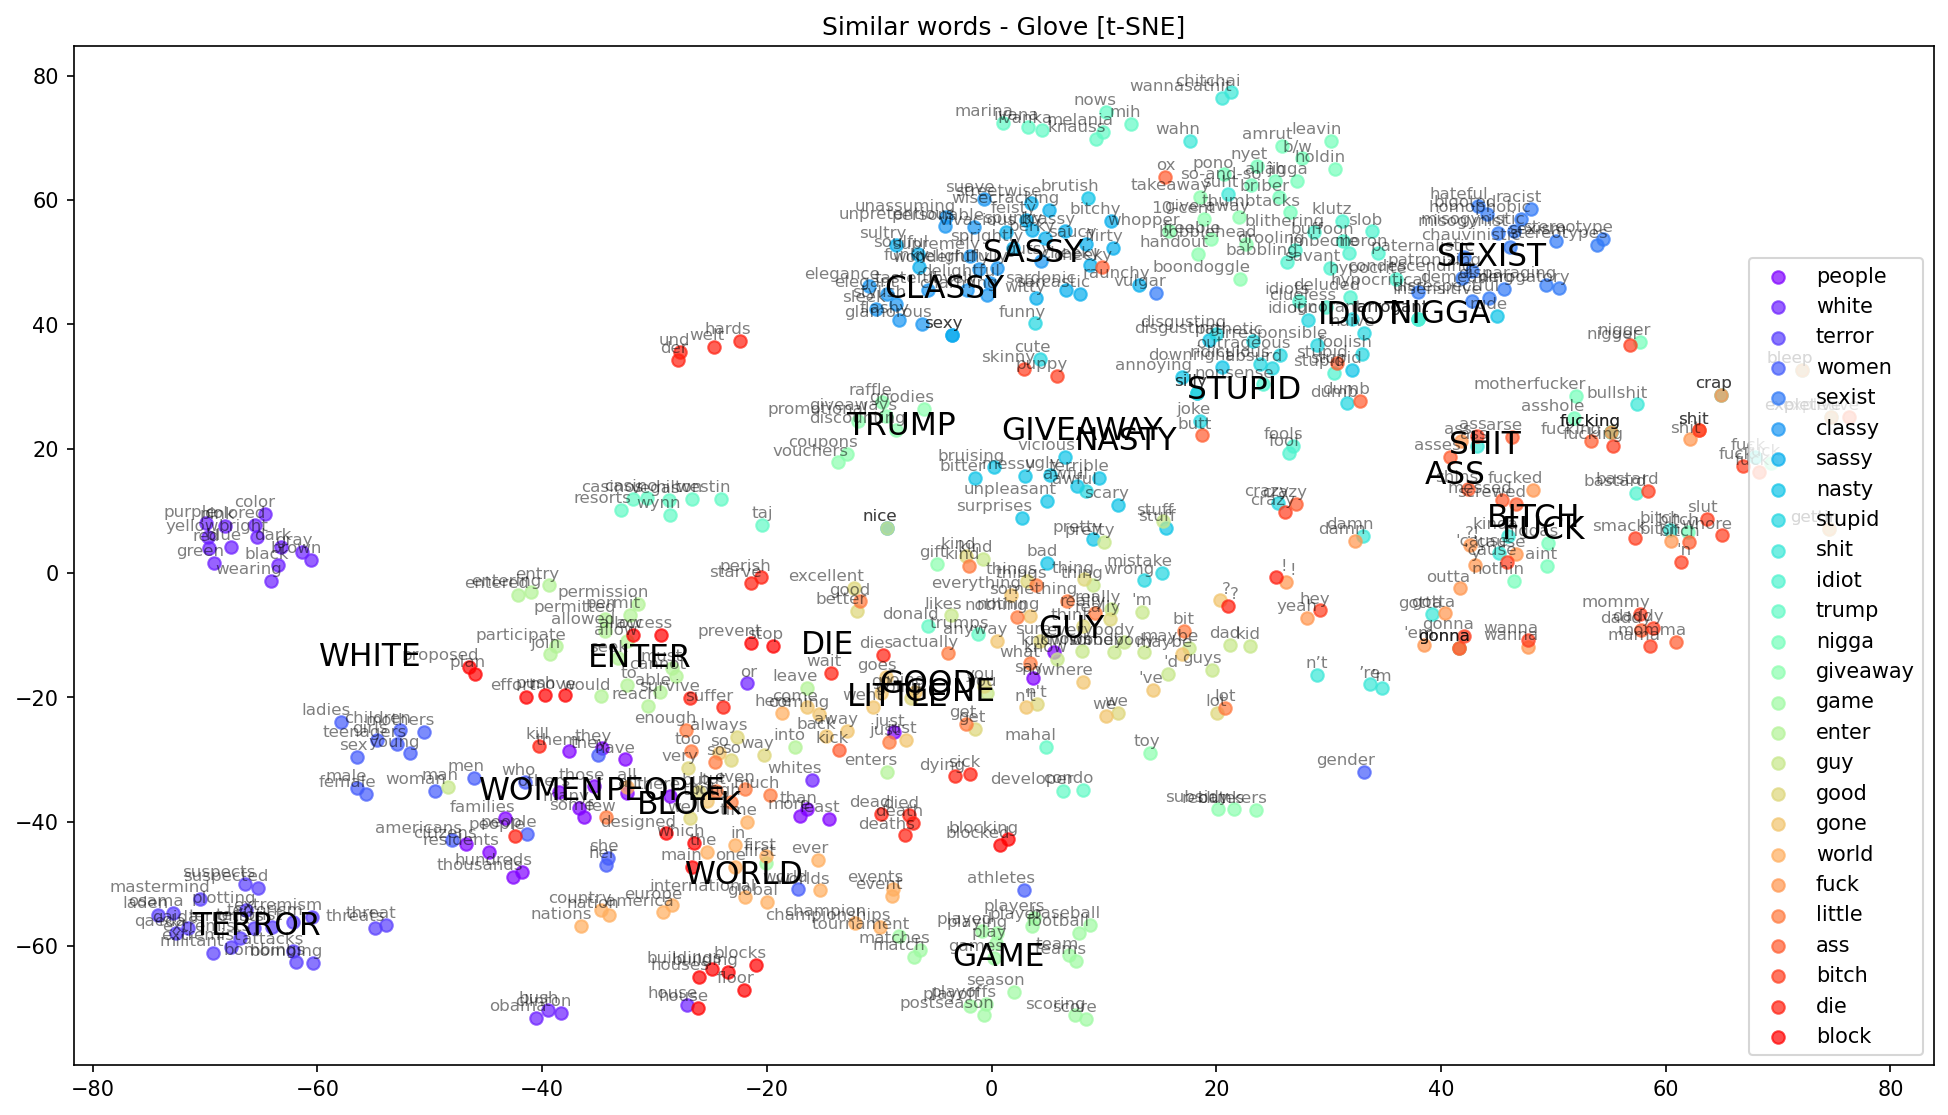
\includegraphics[width=0.495\linewidth]{SimilarWords - Glove - t-SNE.png}
%	\caption{\textbf{Word2Vec and Glove similar words.} Left figure shows Word2Vec embeddings of neighboring words of top unigrams from Table \ref{tab:tf-idf} and the right figure shows Glove embeddings.}
%	\label{fig:embedding_words}
%\end{figure*}

We show the results in Figure~\ref{fig:embedding_labels}. We can see that \textit{homophobic} and \textit{racist} appear very intertwined in Word2Vec and GloVe embeddings, meaning that they cannot be separated, thus indicating a strong relation. On the other hand, in both of these embeddings \textit{spam}, \textit{toxic}, and \textit{discredit} are well separated from other groups and are clearly distinguishable from others. We can also see that \textit{abusive} is entangled with \textit{benevolent} in GloVe representation, however, in results obtained from Word2Vec  \textit{benevolent} is nicely separable from other labels. So it is difficult to conclude that \textit{benevolent} is a label that is different enough from other labels. FastText also nicely separates \textit{toxic} and \textit{benevolent} from other labels, but is unable to separate \textit{vulgar}, \textit{profane} and \textit{obscene}, and \textit{insult}. From all three models combined, we can conclude that the only label that can be always well distinguished from the others is \textit{toxic}, and that \textit{vulgar}, \textit{profane}, \textit{obscene}, and \textit{insult} are labels that cannot be nicely separated. We also conclude that \textit{spam} is a nicely separable category. Note that in some models we omit labels that are not in a vocabulary.


\begin{figure}[!t]
	\centering
	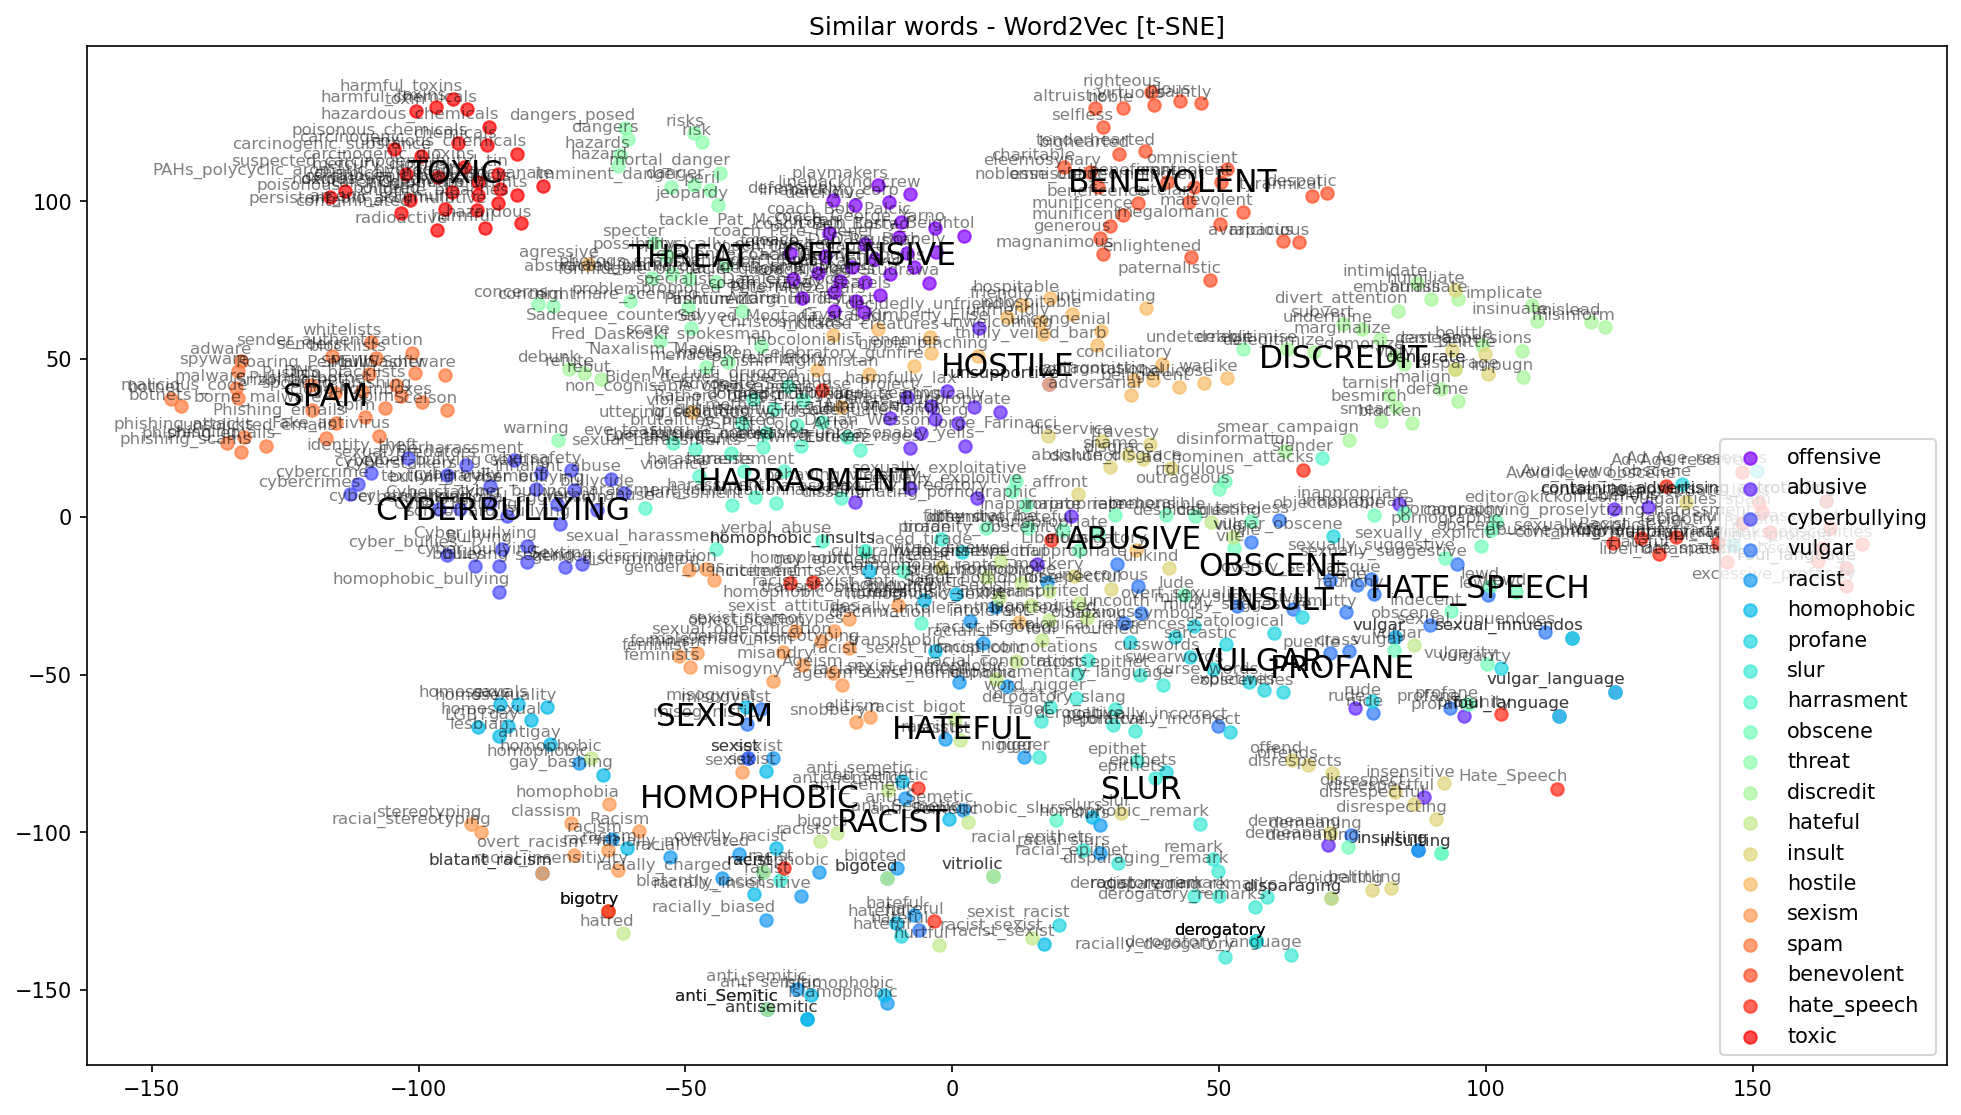
\includegraphics[width=\linewidth]{SimilarWords - word2vec - t-SNE_1.png}
	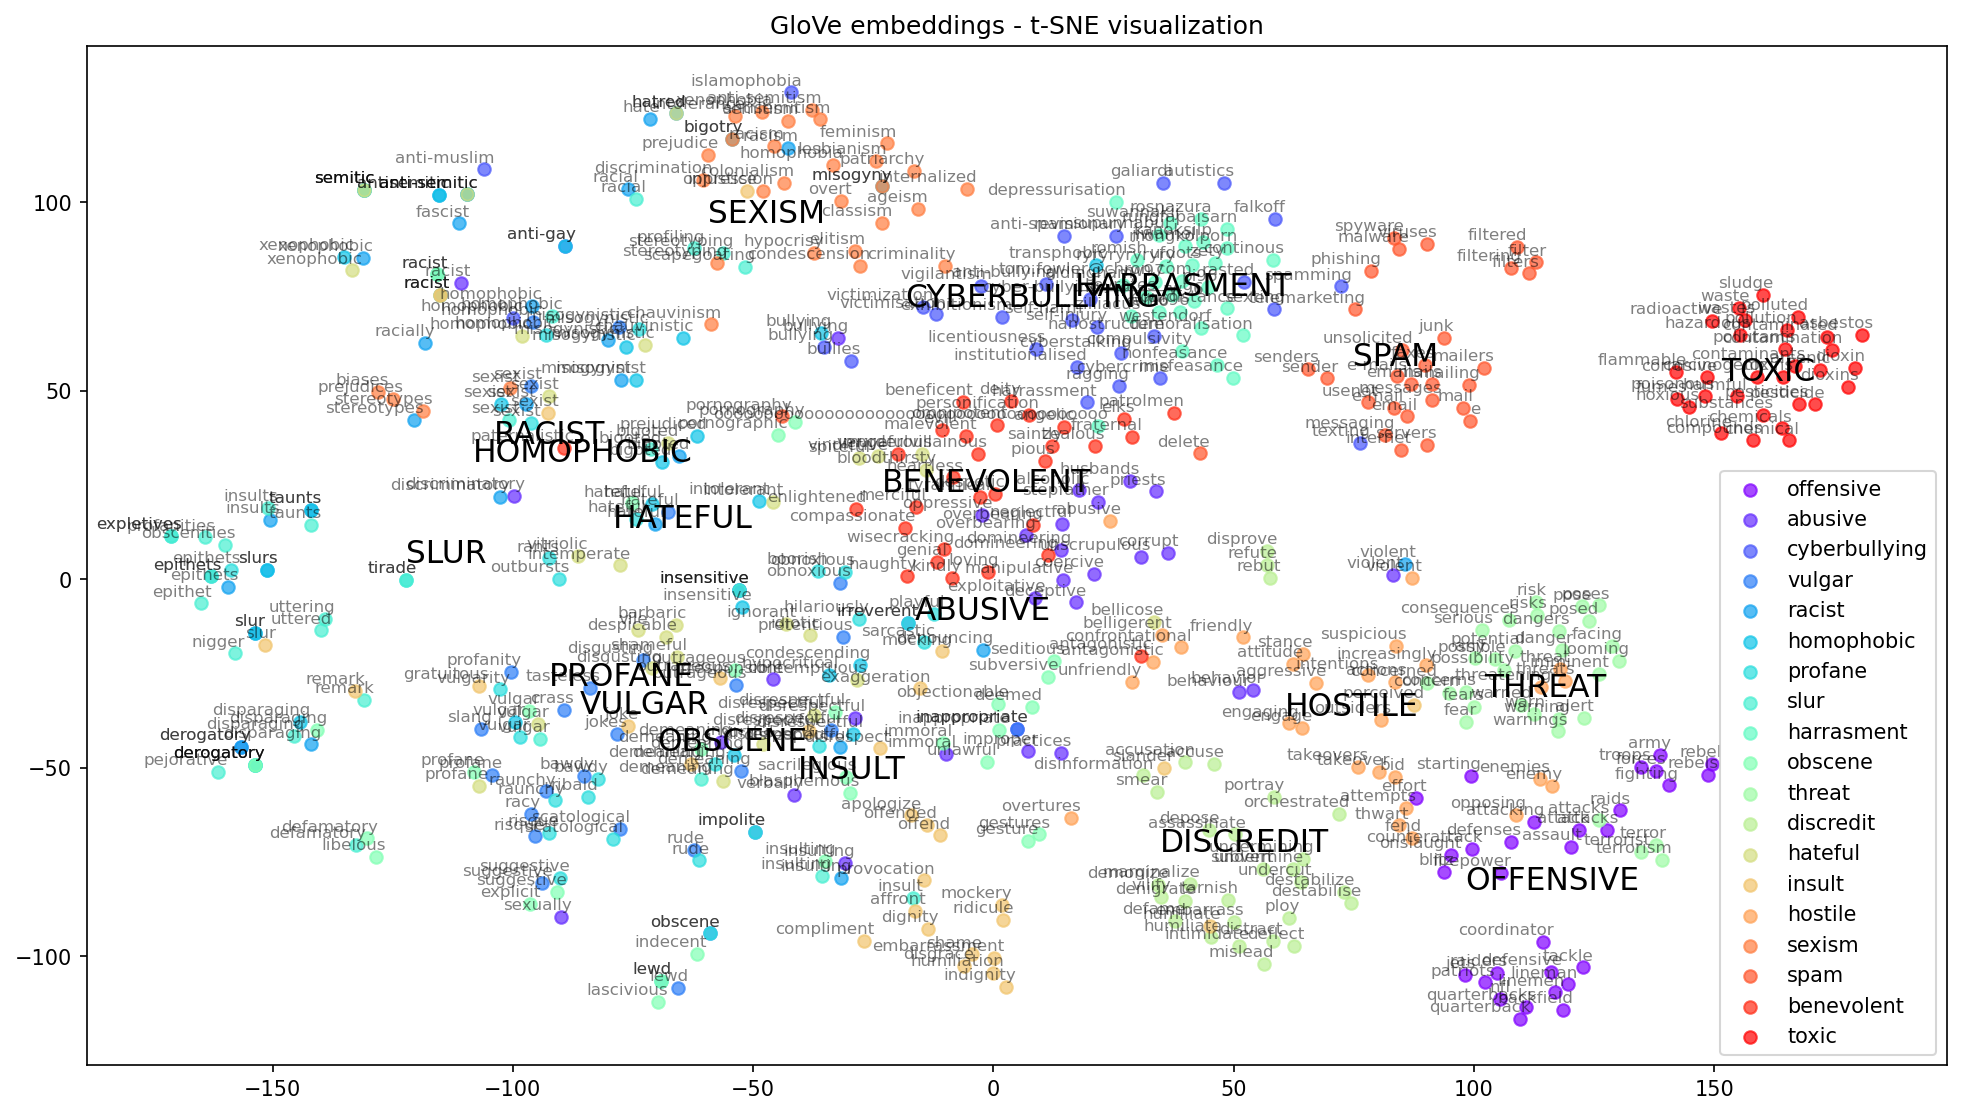
\includegraphics[width=\linewidth]{SimilarWords - Glove - t-SNE_1.png}
	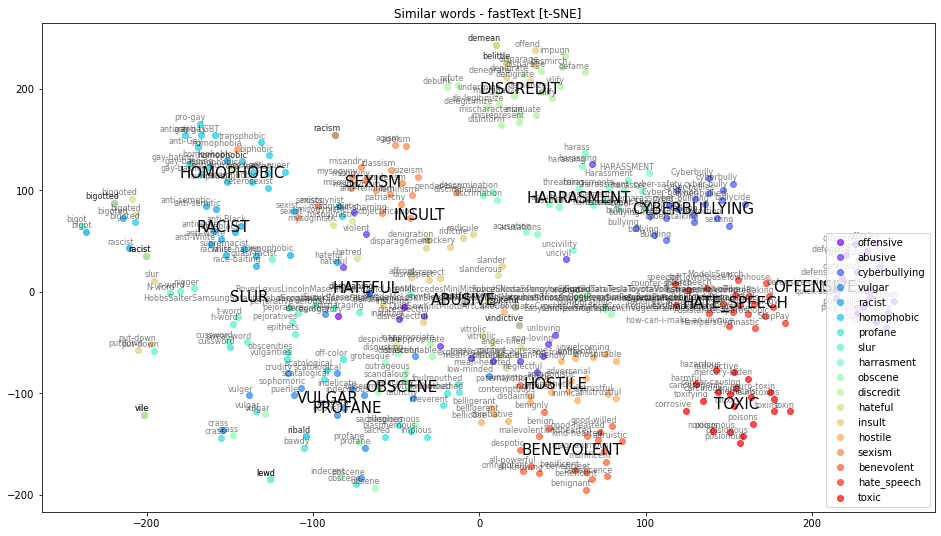
\includegraphics[width=\linewidth]{SimilarWords - FastText - t-SNE_1.png}
	\caption{\textbf{Word2Vec, GloVe, and FastText similar labels.} Figure shows Word2Vec (1st row), GloVe (2nd row), and FastText (3rd row) embeddings of neighboring words of labels we analyze. Note that we omit hate speech subgroups that are not in the vocabulary.}
	\label{fig:embedding_labels}
\end{figure}

By now we provide some relations and decide to further investigate the connections between the related labels using word analogy. We try to find hyponyms and hypernyms, which we do with the help of the following setting:
\begin{verbatim}
father : son = our_label : x 	(hyponyms)
animal : cat = our_label : x 	(hyponyms)
son : father = our_label : x 	(hypernyms)
cat : animal = our_label : x 	(hypernyms)
\end{verbatim},
where \texttt{our\_label} is one of the analyzed labels and \texttt{x} is the word found by Word2Vec or GloVe. 

Unfortunately, the relationships are not clear and uniquely defined. An example is \textit{racism} is to \textit{sexism} what is \texttt{son} to \texttt{father} with $\approx 64.6\%$ probability, but \textit{sexism} is to \textit{racism} what is \texttt{son} to \texttt{father} with $\approx 64.8\%$ probability. We can once again see that the two labels are related, but the precise relationship cannot be inferred. Using \texttt{brother} and \texttt{sister} the probability is lower. This could indicate that it is impossible to find a specific hypernym and that we can only conclude that the labels are more closely related to each other, as they are each in some way hypernym and hyponym of each other. Similarly, \textit{racism} and \textit{sexism} are connected to \textit{homophobia} and \textit{slur}. Another group that we find, but also cannot clearly define the inner relations contains \textit{vulgar}, \textit{profane}, and \textit{obscene}.

As mentioned, the distances between the inspected labels cannot be determined from our chosen visualization. That is why we approach this problem with clustering. We use $k$-means and hierarchical clustering in hopes of finding meaningful clusters that could help us understand the relationships between the subgroups of the hate speech better. We determine the $k$ in $k$-means by using the silhouette score. Note that we choose the $k$ of the second peak of the score, as we want to form more diverse and meaningful clusters than just $2$ big subgroups as the silhouette score suggests. See the example output of the silhouette score in Figure \ref{fig:silh}.

\begin{figure}[htb]\centering
	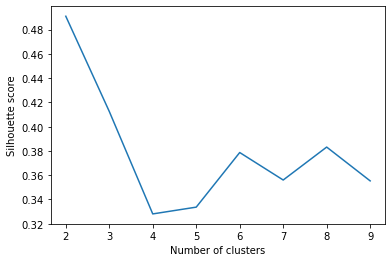
\includegraphics[width=\linewidth]{silh.png}
	\caption{\textbf{Silhouette score.} Example of silhouette scores for different numbers of clusters. We use the second peak ($k = 6$) instead of first ($k = 2$), as we want to get more clusters.}
	\label{fig:silh}
\end{figure}

From the top 30 similar words for each label, we compute an average vector and we obtain one such vector for each label. We compute the cosine similarity matrix between the vectors $simcos$ and compute the distance matrix as $d = 1 - simcos$, which we then use for the clustering. In Table \ref{tab:clustering_labels_word2vec} we show the obtained clusters and in Figure \ref{fig:hier} we show the results of hierarchical clustering of Word2Vec embeddings.

From these two clustering results we can infer that \textit{insult} and \textit{obscene} are two similar subgroups of hate speech as they both appear in the same cluster in+ $k$-means clustering and we can see that they are closely together in hierarchical clustering. They are also very similar according to the results from TF--IDF as seen before. \textit{Benevolent sexism} is also close. We can see that \textit{cyberbullying} and \textit{spam} are clustered together in both clusterings and that \textit{threat} and \textit{toxic} are also very similar. From the results of hierarchical clustering we can see that \textit{offensive} is also close to them.

\begin{figure}[htb]\centering
	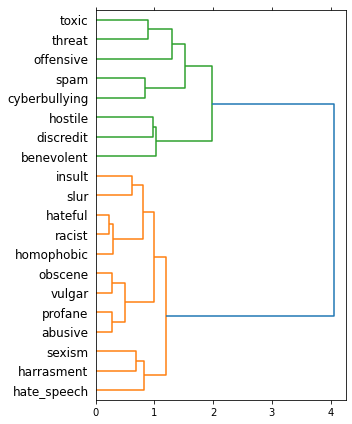
\includegraphics[width=0.6\linewidth]{hier.png}
	\caption{\textbf{Hierarchical clustering of average Word2Vec embeddings of labels' $30$ nearest words.} Figure shows results of hierarchical clustering of the labels from data sets. Distance between two labels is computed as $1 - simcos$, where $simcos$ is a cosine similarity between two labels. Embedding for each label is computed as an average of embeddings of label's nearest $30$ words.}
	\label{fig:hier}
\end{figure}

Comparing the hierarchical clustering results of GloVe and FastText embeddings to Word2Vec embeddings, we can see that we always get almost the same two main clusters as those in Figure \ref{fig:hier}, so we do not show figures with those results. 

Looking at $k$-means clustering of Word2Vec and GloVe embeddings we see that pairs of \textit{abusive}, \textit{vulgar}, \textit{racist}, \textit{homophobic}, \textit{profane}, \textit{slur}, \textit{obscene}, \textit{hateful} and \textit{insult}, and \textit{discredit} and \textit{hostile} always appear in the same two clusters, so we can conclude that they are related. We do not include the results of FastText $k$-means clustering, as its silhouette score is $\le 0.30$ for all possible $k$, whereas in the first two, the score is often $> 0.30$. 

We try to apply this same approach to the words with highest TF--IDF scores from each subgroup, however, the obtained clusters provide no useful understanding, so we omit those results.

\begin{table}[htb]
\scriptsize
\centering
\begin{tabular}{c|l}
\toprule
\textbf{cluster} & \textbf{components}                                                                                                                                        \\ \midrule
1                & offensive                                                                                                                                                  \\ \hline
2                & \begin{tabular}[c]{@{}l@{}}abusive, vulgar, racist, homophobic, profane, \\ slur, harassment, obscene, hateful, insult,\\ sexism, hate speech\end{tabular} \\ \hline
3                & discredit, hostile, benevolent                                                                                                                             \\ \hline
4                & cyberbullying, spam                                                                                                                                        \\ \hline
5                & threat, toxic                                                                                                                                              \\ \bottomrule
\end{tabular}
\caption{\textbf{$K$-means clustering of average Word2Vec embeddings of labels' 30 nearest words.} Table shows five clusters obtained with 5-means clustering. We determine $k = 5$ using silhouette score.}
	\label{tab:clustering_labels_word2vec}
\end{table}


\begin{figure}[htb]\centering
	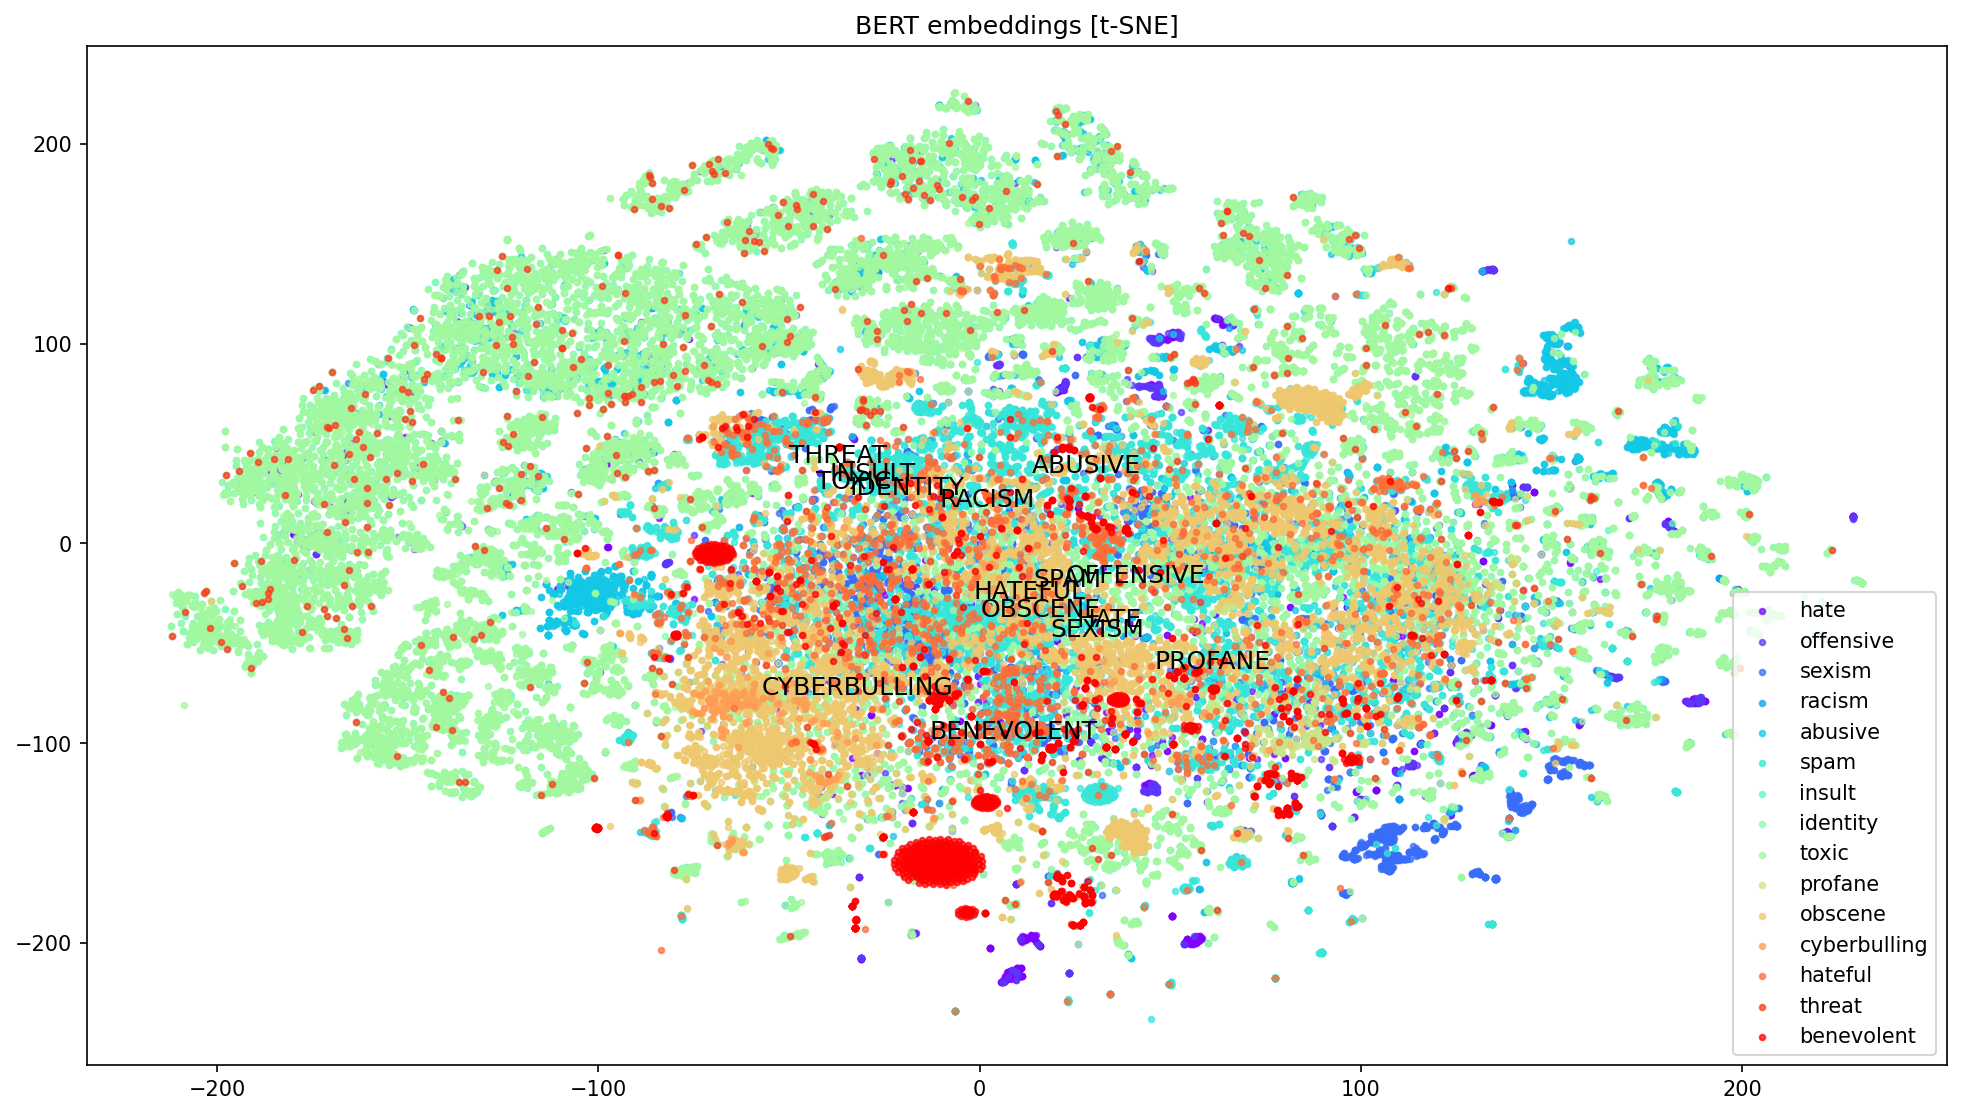
\includegraphics[width=\linewidth]{bert_tsne.png}
	\caption{\textbf{BERT embeddings.} T-SNE visualization of BERT embeddings of labels.}
	\label{fig:berttsne}
\end{figure}

% ------------------------- contextual -------------------------------------
\subsection{Contextual word embeddings}

% --------------------------------------------------------------
\subsubsection{BERT}
We move on to contextual embeddings and we focus on BERT. We use the pretrained BERT base cased model \cite{dbpl} and convert tweets and comments from our data set to BERT embeddings. We first append them "\texttt{ - This is <label>}" and compute the embeddings. From obtained embeddings of each vector, we compute an average representation from the vectors that belong to the tokens of the \texttt{label}. We average the obtained representation of each label and use cosine similarity to compute the similarity between those label representations. We show the obtained similarity matrix in Figure \ref{fig:bertsim1}. We can see high similarities between most of the subgroups of hate speech. The one that differs the most from the other groups is \textit{cyberbullying}. We can also see that \textit{profane} is slightly less similar to \textit{identity}, \textit{insult}, \textit{threat}, and \textit{toxic}, however, the similarity score is still between $0.87$ and $0.89$. For all other combinations the similarity score is $\ge 0.90$. We also visualize the embeddings with the help of t-SNE in Figure \ref{fig:berttsne} and we show the labels on the mean points of each subgroup. We can see that all subgroups are tightly connected and it is hard to distinguish between them. However, we can see that \textit{cyberbullying} is a little bit more compact and not as dispersed as others, which might be a reason behind slightly different similarity scores. It is also interesting that some labels, although being dispersed, have some small clusters which stand out and might indicate special subgroups within those subgroups of hate speech. Example of such subgroup is \textit{benevolent sexism}.

\begin{figure}[htb]\centering
	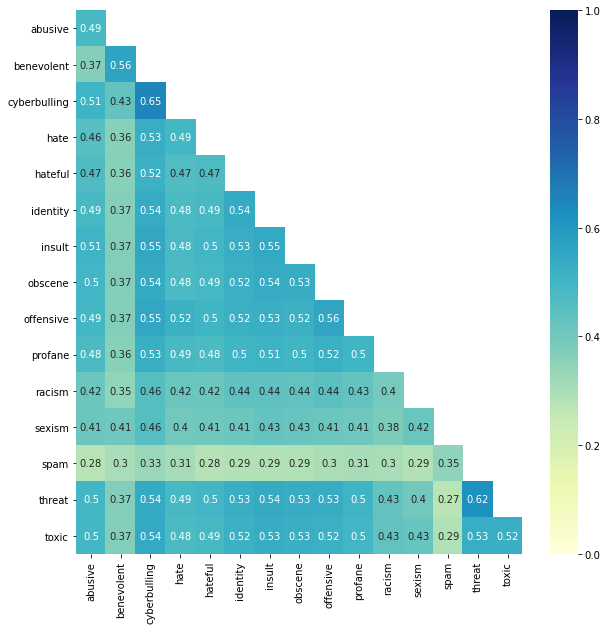
\includegraphics[width=0.9\linewidth]{bert_sim1.png}
	\caption{\textbf{Similarities between BERT embeddings.} Figure shows similarity between labels' BERT embeddings. For each label we obtain an average vector representation by averaging embeddings obtained from label's tweets / comments. Similarity is  then computed as a cosine similarity between those vector representations.}
	\label{fig:bertsim1}
\end{figure}

\subsubsection{KeyBERT}
We leverage the KeyBERT \cite{grootendorst2020keybert}, which is a minimal keywords extraction technique that uses BERT embeddings to create keywords and keyphrases that are most similar to a document. For each label we compute top $3$ keywords for each tweet / comment using KeyBERT, and show the labels' $5$ most common keywords in Table \ref{tab:bertkey}. We can see that \textit{insult}, \textit{obscene}, and \textit{toxic} have the same $5$ most common keywords. Since they come from the same data set, and since each tweet from that data set could have multiple labels, we feel that this affected the results. We can see that quite a few labels include common keywords such as fuck, bitch, fucking, and idiot, which is not surprising, as they are among the top common curses. We can see more Trump related words in \textit{offensive}, \textit{profane}, \textit{hate speech}, which is probably again due to the background of data set generation. However, the most common keyword sets of those labels still slightly differ. Keywords are the most diverse between \textit{benevolent}, \textit{cyberbullying}, \textit{racism}, \textit{sexism}, and \textit{spam}.


\begin{table}[]
\scriptsize
\centering
\begin{tabular}{l|l}
\toprule
\textbf{category} & \textbf{BERT keywords}                                                                                                                                \\ 
\midrule
racism            & \begin{tabular}[c]{@{}l@{}}coon, white, black, terror, fuck\end{tabular}                \\ \hline
sexism            & \begin{tabular}[c]{@{}l@{}}sexist, women, feminazi, girls, kat\end{tabular}                                 \\ \hline
benevolent        & \begin{tabular}[c]{@{}l@{}}women, womensday, sassy, \\adaywithoutwomen, woman\end{tabular}                \\ \hline
abusive          & \begin{tabular}[c]{@{}l@{}}fucking, idiot, bitch, hate, fuck\end{tabular}                      \\ \hline
hateful          & \begin{tabular}[c]{@{}l@{}}hate, trump, idiot, nigga, fucking\end{tabular}              \\ \hline
spam              & \begin{tabular}[c]{@{}l@{}}video, new, 2017, liked, free\end{tabular}                                      \\ \hline
cyberbullying    & \begin{tabular}[c]{@{}l@{}}riot, troll, hacking, trolls, hacker\end{tabular}                  \\ \hline
hate speech       & \begin{tabular}[c]{@{}l@{}}trumpisatraitor, doctorsfightback, shameonicc, \\borisjohnsonshouldnotbepm, trump\end{tabular} \\ \hline
identity hate     & \begin{tabular}[c]{@{}l@{}}gay, fuck, nigger, bitch, fucking\end{tabular}                                          \\ \hline
insult           & \begin{tabular}[c]{@{}l@{}}fuck, wikipedia, bitch, fucking, suck\end{tabular}                            \\ \hline
obscene          & \begin{tabular}[c]{@{}l@{}}fuck, wikipedia, bitch, fucking, suck\end{tabular}                            \\ \hline
offensive        & \begin{tabular}[c]{@{}l@{}}trumpisatraitor, fucktrump, trump, murderer, rapist\end{tabular}            \\ \hline
profane          & \begin{tabular}[c]{@{}l@{}}fucktrump, fuck, dickhead, trump, douchebag\end{tabular}  \\ \hline
threat            & \begin{tabular}[c]{@{}l@{}}kill, die, fuck, bitch, rape, death\end{tabular}                                           \\ \hline
toxic            & \begin{tabular}[c]{@{}l@{}}fuck, wikipedia, bitch, fucking, suck\end{tabular}   
\\
\bottomrule                       
\end{tabular}
\caption{\textbf{BERT keywords.} Table shows 5 most important keywords for each hate speech subgroup found with BERT. Note: categories that have an $\*$ contain also 2 keywords (dumbdonnythedraftdodgingdotart and worstsecretaryofstateinushistory) but we omit them in order to obtain clearer represenatation of categories.}
\label{tab:bertkey}
\end{table}

\subsubsection{Universal Sentence Encoder}
We additionally use one approach that was not suggested and that is Universal Sentence Encoder (USE) which is a model that can be nicely used for semantic similarity. As we are interested in the relations and connections between subgroups of hate speech, we try to use this model to further analyze the structure of hate speech in general.

We average the obtained representation of each label and use cosine similarity to compute the similarity between those label representations. We show the obtained similarity matrix in Figure \ref{fig:use_sim}

From the plot we can see that similarly to BERT results, the subgroups here are again very similar. However, we can find some subgroups, that are still a little bit less similar. One example is \textit{hateful} that is less similar to other groups, and the most similar to \textit{spam} and \textit{abusive}. Consequently, \textit{abusive} is more similar to \textit{hateful} and \textit{spam} and a little bit less similar to others. Same holds for \textit{spam}, which is more similar to  \textit{hateful} and \textit{abusive} than to others. From this we can infer that  \textit{hateful}, \textit{abusive}, and \textit{spam} are $3$ subgroups of hate speech that are tightly connected to each other, and less connected to all other subgroups.
\begin{figure}[htb]\centering
	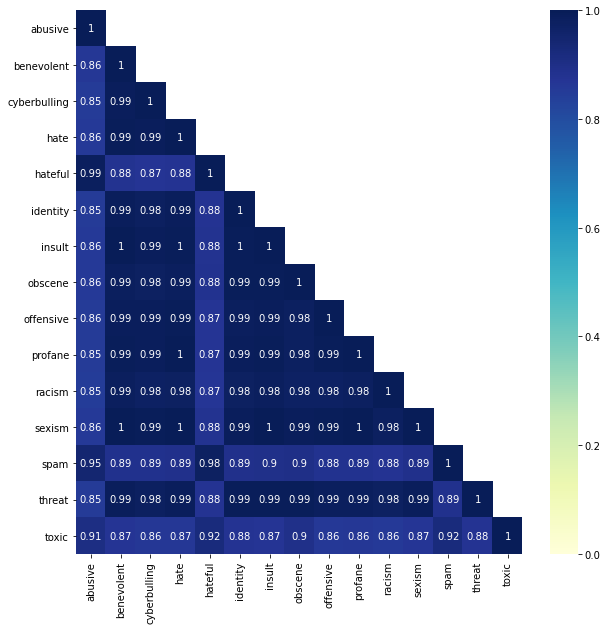
\includegraphics[width=0.9\linewidth]{use_sim.png}
	\caption{\textbf{Similarities between USE embeddings.} Figure shows similarity between labels' USE embeddings. For each label we obtain an average vector representation by averaging embeddings obtained from label's tweets / comments. Similarity is  then computed as a cosine similarity between those vector representations.}
	\label{fig:use_sim}
\end{figure}


% -------------------------------------------------------------------------------
\section{Schema}
\label{sec:schema}
Considering all the results and findings from above, we can now provide the following inference. Note that all categories are tightly connected in contextual embeddings, which should be kept in mind. However, we want to provide some sort of separation where possible, so we consider more the results that separated our subcategories of hate speech. We can define the following "blocks", that contain the subgroups of hate speech in one island are connected to each other more than to subgroups from other islands. Those subgroups, that are an island by themselves, are the subgroups that can be nicely separated from all other subgroups. 

\begin{enumerate}
  \item \textit{sexism}, \textit{racism}, \textit{homophobic}, and \textit{slur};
\vspace{-10pt} 
  \item \textit{obscene}, \textit{insult}, \textit{profane}, \textit{abusive}, \textit{vulgar};
\vspace{-10pt}
  \item \textit{discredit, offensive, hostile, threat, benevolent};
\vspace{-10pt}
  \item \textit{spam};
\vspace{-10pt}
  \item \textit{cyberbullying}.
\end{enumerate}

The above list includes $16$ out of $21$ subgroups that we analyze. The reason behind is that \textit{hate speech} is a subgroup that can be connected with blocks $1$ and $2$. Similar holds for \textit{hateful}, which can be connected to the first $3$ blocks, however, it is never connected to \textit{abusive}. Another subgroup that is sometimes connected to block $1$ is \textit{harassment}. 

As we see that some subgroups cannot be separated just yet (block $1$, $2$, and $3$), we apply further analysis with Word2Vec and GloVe. We focus on the labels and use the embeddings of their $50$ most similar words. For the three of the following figures we use PCA visualization, so that we can also see the distance between subgroups. In the first plot of Figure \ref{fig:further1} we see that \textit{racism}, \textit{slur}, and \textit{homophobic} are more related to each other than to \textit{sexism}. In the second plot of Figure \ref{fig:further1} we can see that all of the inspected subgroups are tightly connected and cannot be nicely separated, \textit{insult}, however, slightly stands out. In the last plot of Figure \ref{fig:further1} we can see that \textit{discredit} is not as intertwined with \textit{insult} and \textit{obscene}, so we conclude that although it is related to them, it it still a bit less connected to them, as they are to each other.

\begin{figure*}[htb]\centering
	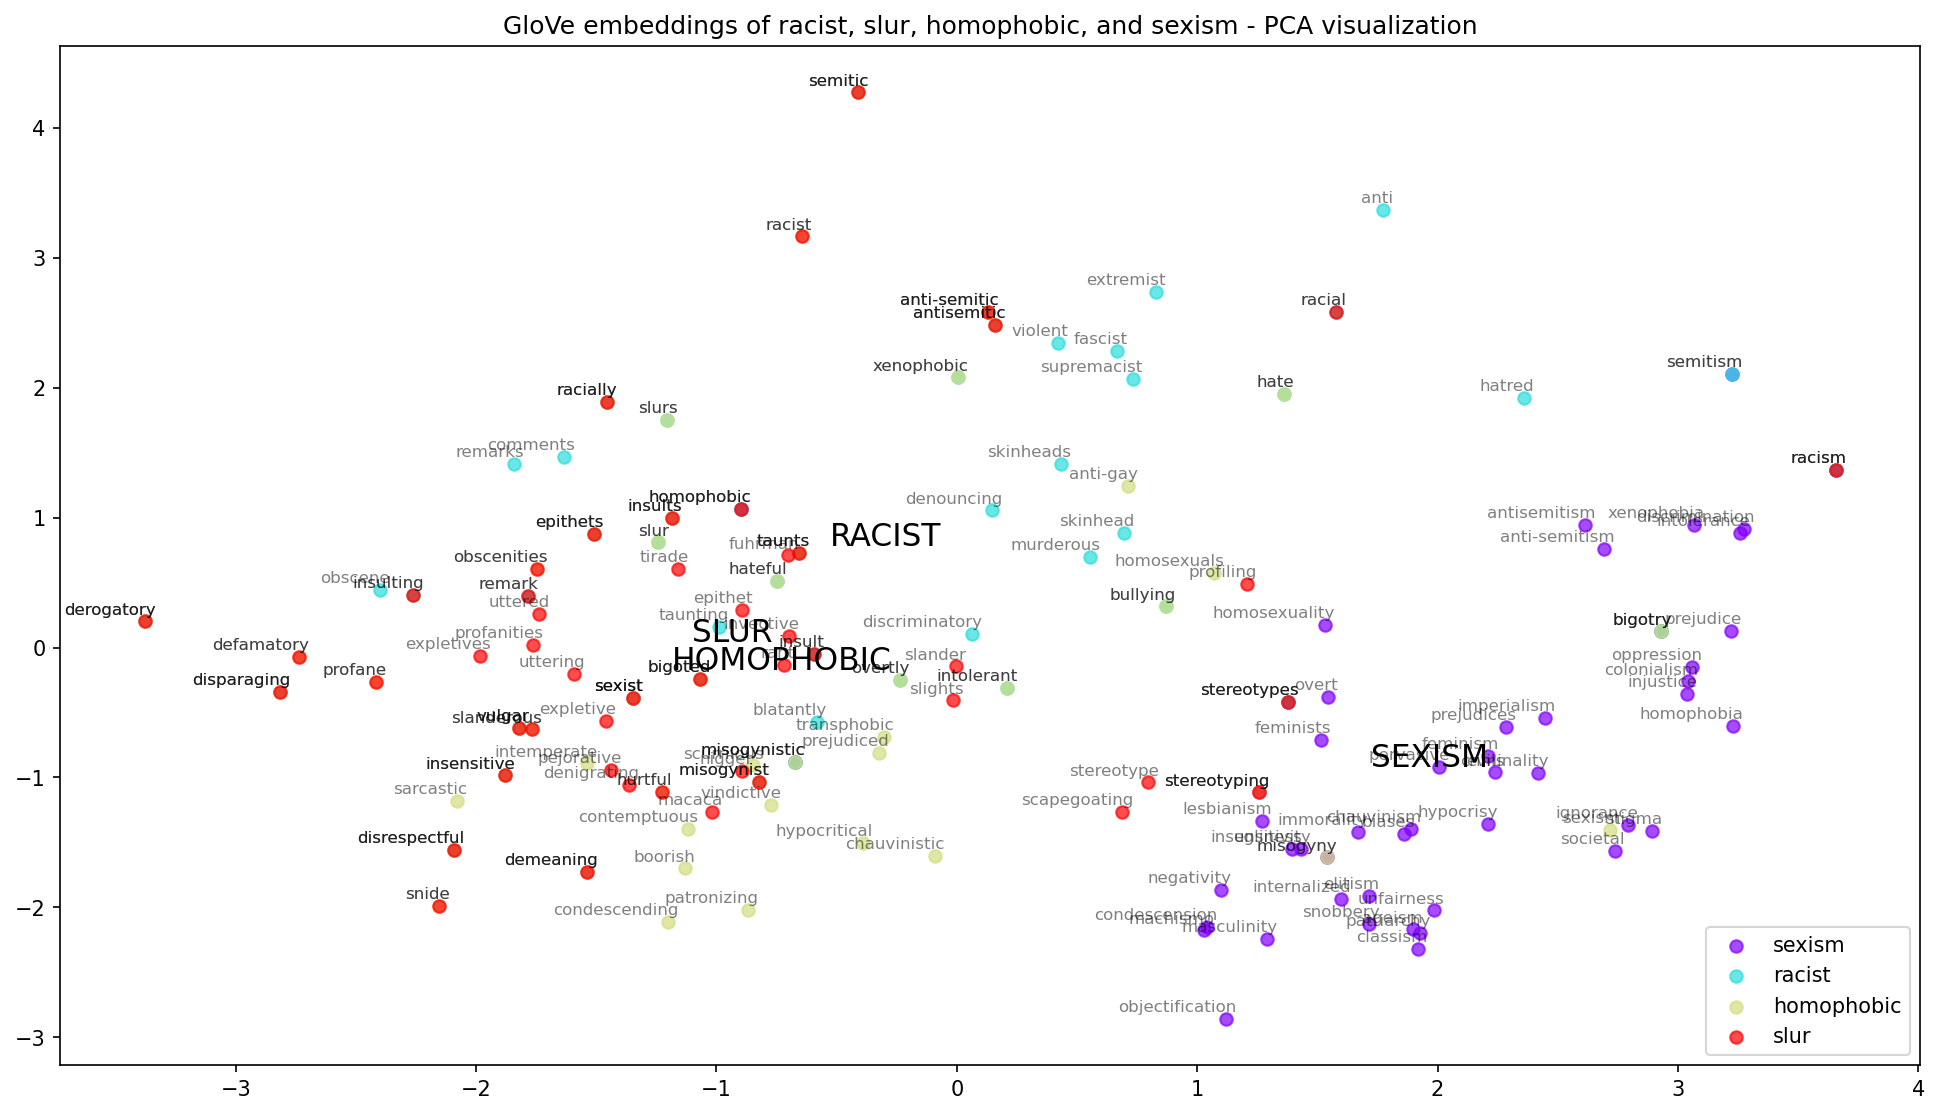
\includegraphics[width=0.33 \linewidth]{Further analysis - Glove - PCA.png}
	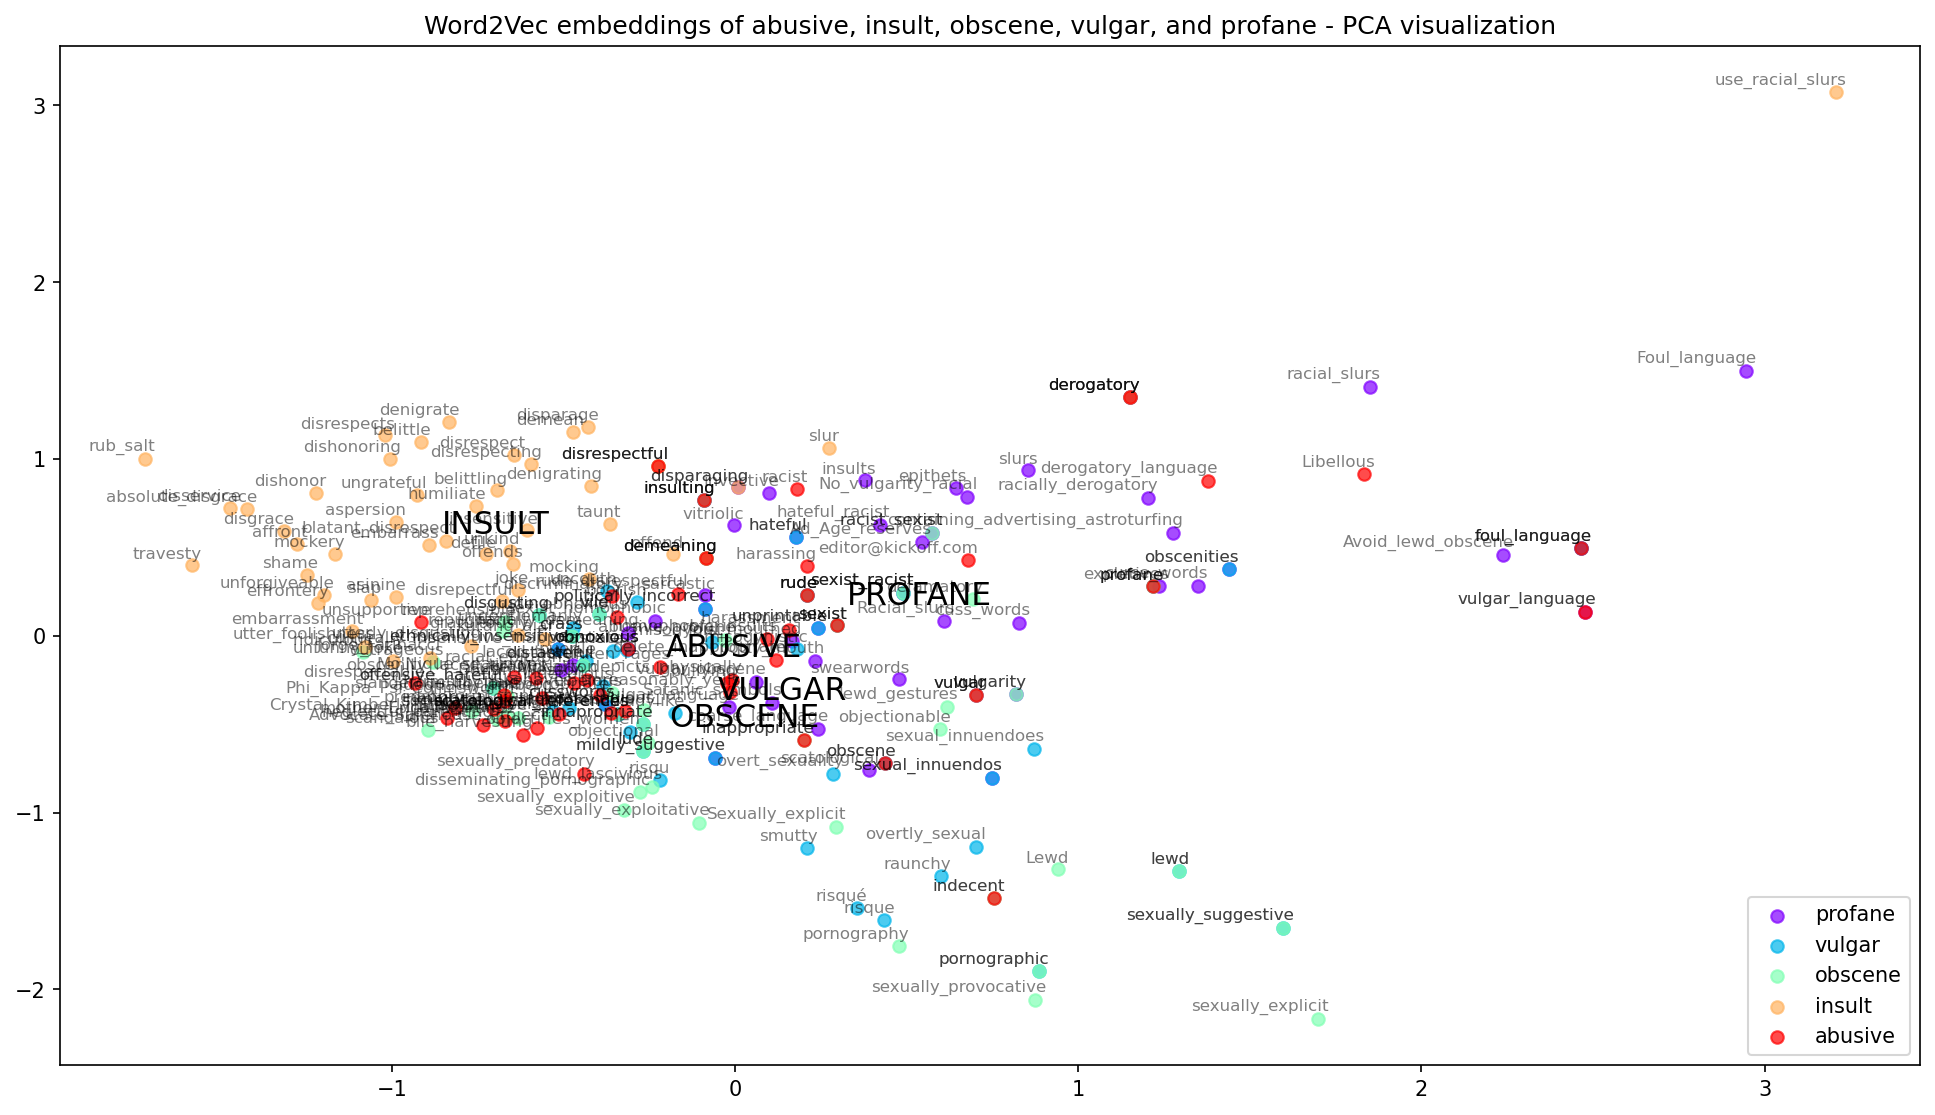
\includegraphics[width=0.33 \linewidth]{Further analysis1 Word2Vec - PCA.png}
	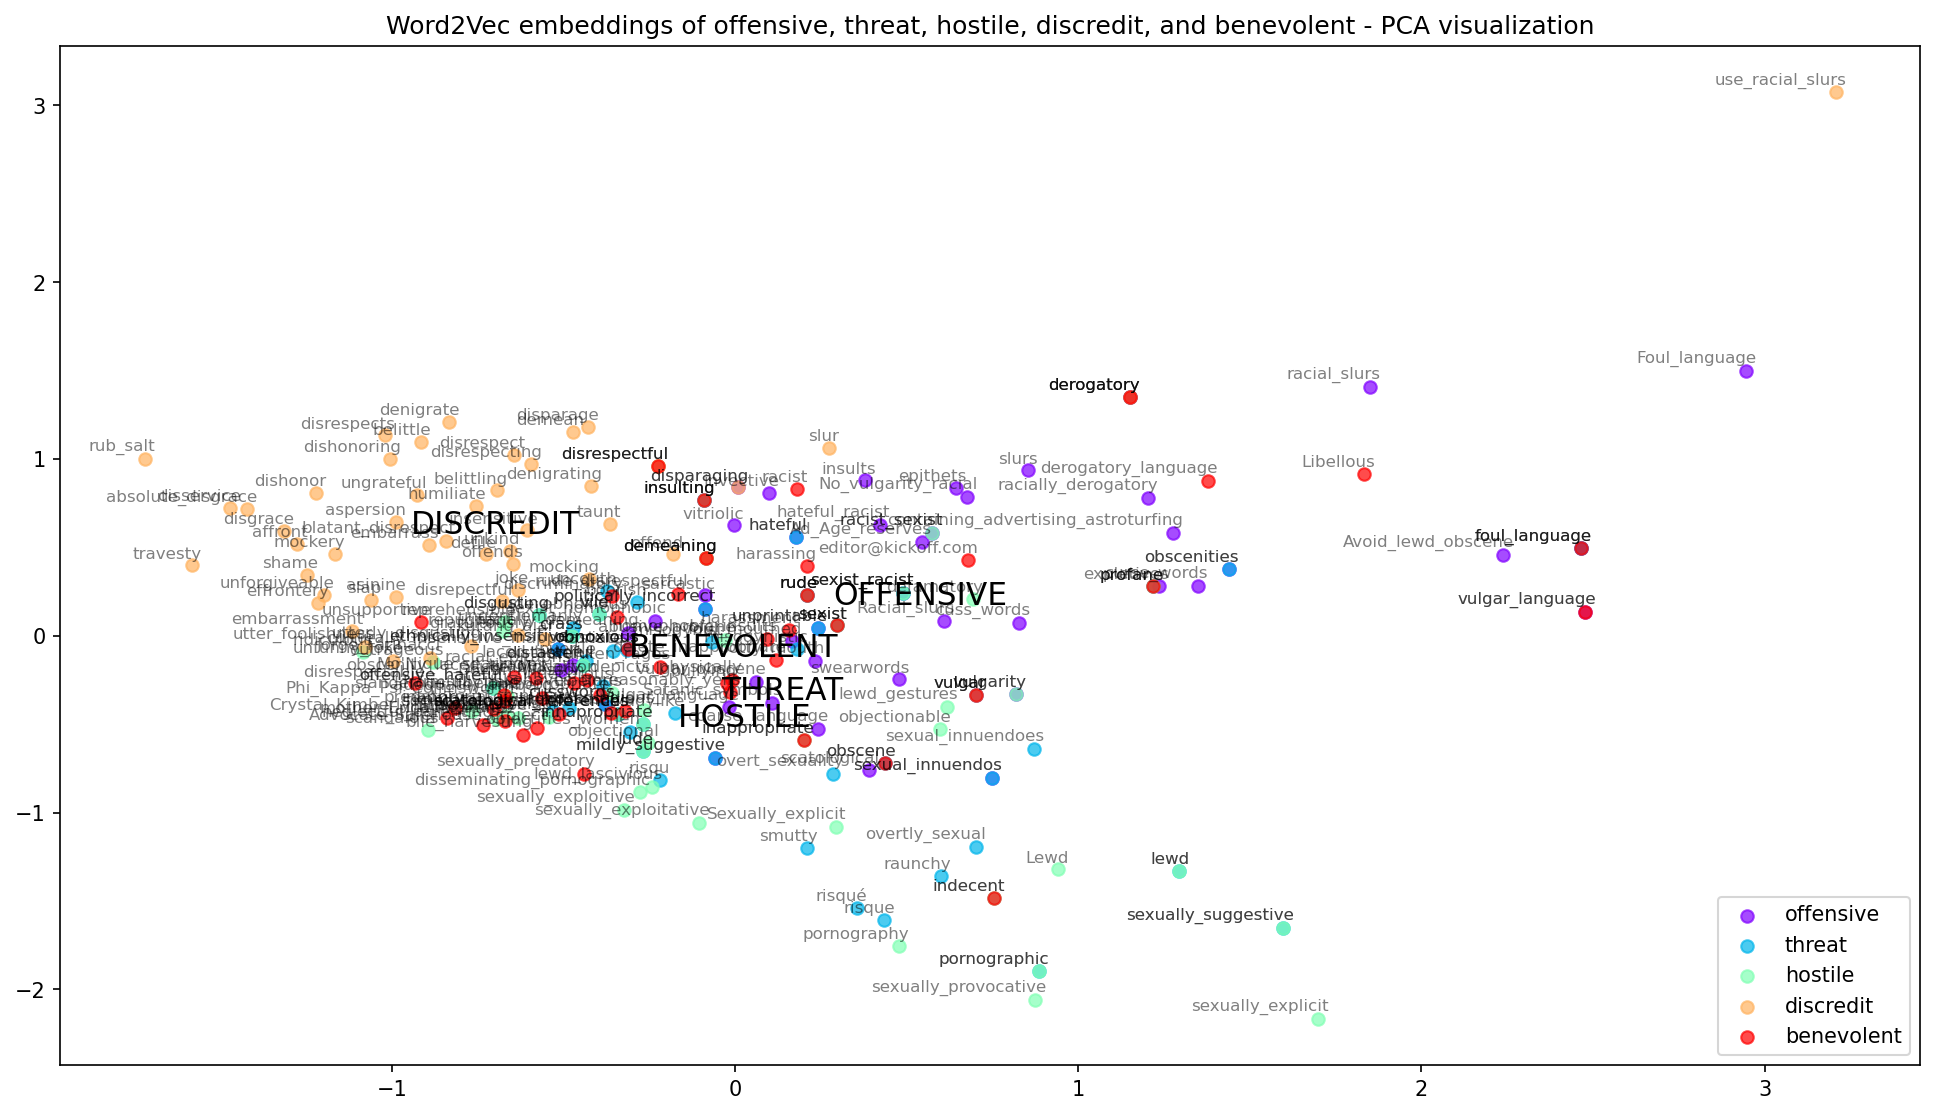
\includegraphics[width=0.33 \linewidth]{Further analysis2 Word2Vec - PCA.png}
	\caption{\textbf{Further analysis of blocks that could not be separated.} We use PCA visualization in all plots and $50$ nearest words' embeddings of each label are used. We use GloVe embeddings in the first plot, and Word2Vec in the other two.}
	\label{fig:further1}
\end{figure*}

From the above findings, we try and provide a schema of hate speech subcategories in Figure \ref{fig:schema}. Note that the schema is obtained with the described analysis and it is not confirmed by any linguist professional. All of the subgroups are also tightly connected, however, as the goal of our paper is try to provide some meaningful relations, we try to summarize our findings in a schema and show more connected groups together. We found $3$ mains groups, that are shown in bordered rectangles. Difference in colors means, that the node is slightly less connected to other nodes in those groups. \textit{Spam} and \textit{cyberbullying} are both gray, as they are connected, but they each could be put in a separate rectangle, as they differ enough. We place them next to \textit{toxic} as slight relations can be seen between those three. \textit{Toxic} and \textit{benevolent} are also connected to some of the nodes in the blue subgroup. The latter is also connected to \textit{hateful}. We also see that \textit{insult} has a strong relation with the red and green subgroups, and \textit{discredit} from the blue. General \textit{hate speech} is mostly connected to the red and green subgroup. Note that \textit{identity hate} is related to all, but we could not find a stronger relation to any specific subgroup.

\begin{figure}[htb]\centering
	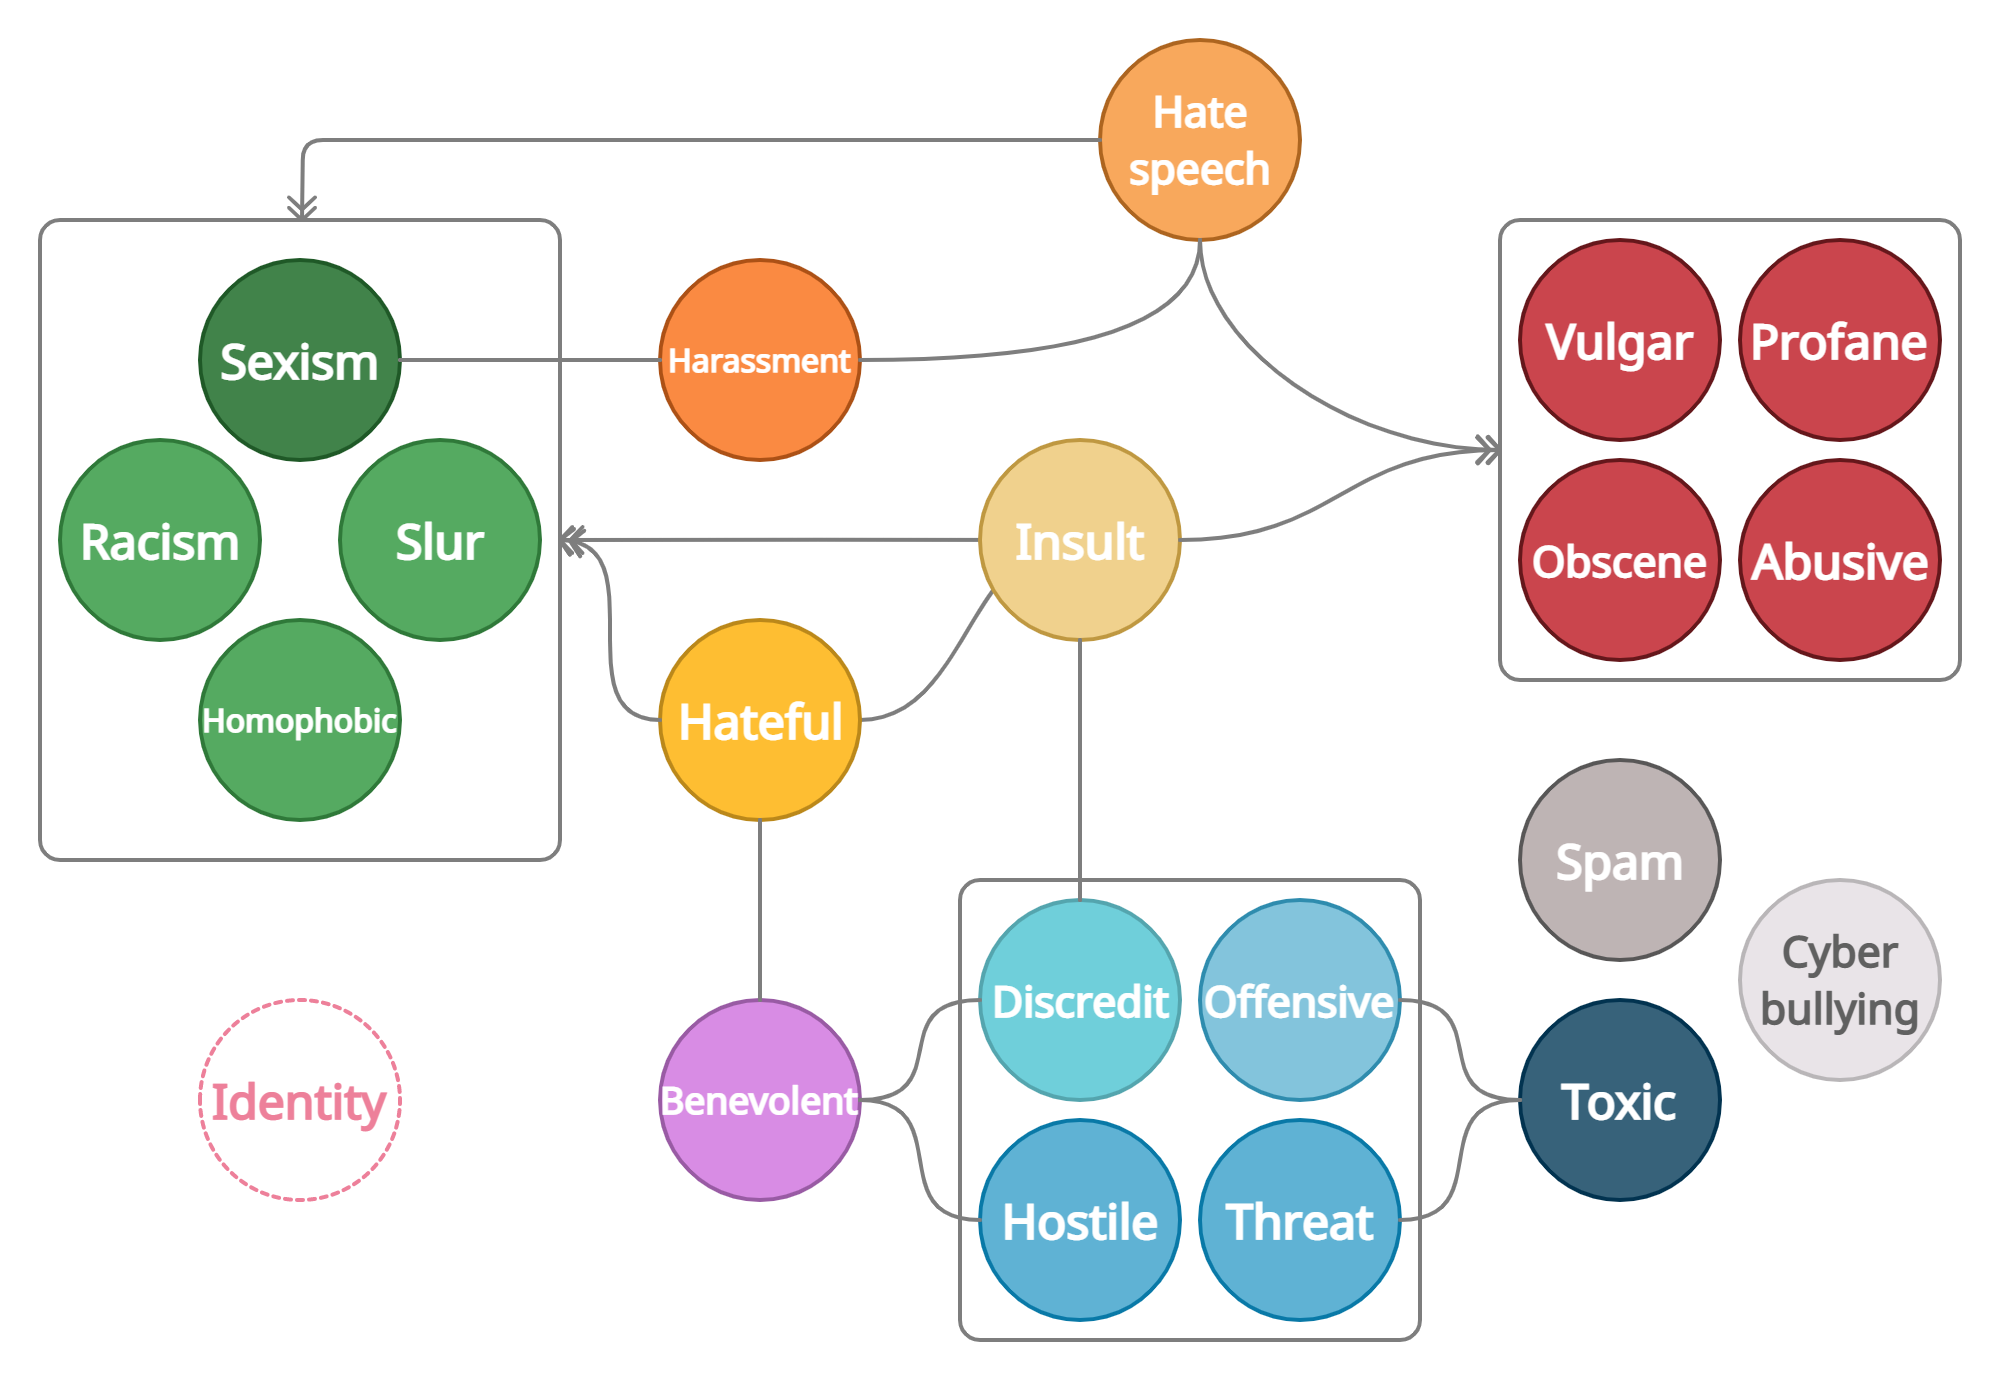
\includegraphics[width= \linewidth]{final_schema.png}
	\caption{\textbf{Proposed schema of hate speech.} Figure shows the proposed schema of hate speech. Note that all of the labels are very related, however, we try to provide one possible division. Nodes in groups that are of slightly different color are more separable from other nodes in this group. We show connections to other the nodes with normal lines and connections to whole groups with line and two arrows. Identity is dotted because we do not have enough information to connect it with other node or group.}
	\label{fig:schema}
\end{figure}

%\begin{figure}[htb]\centering
%	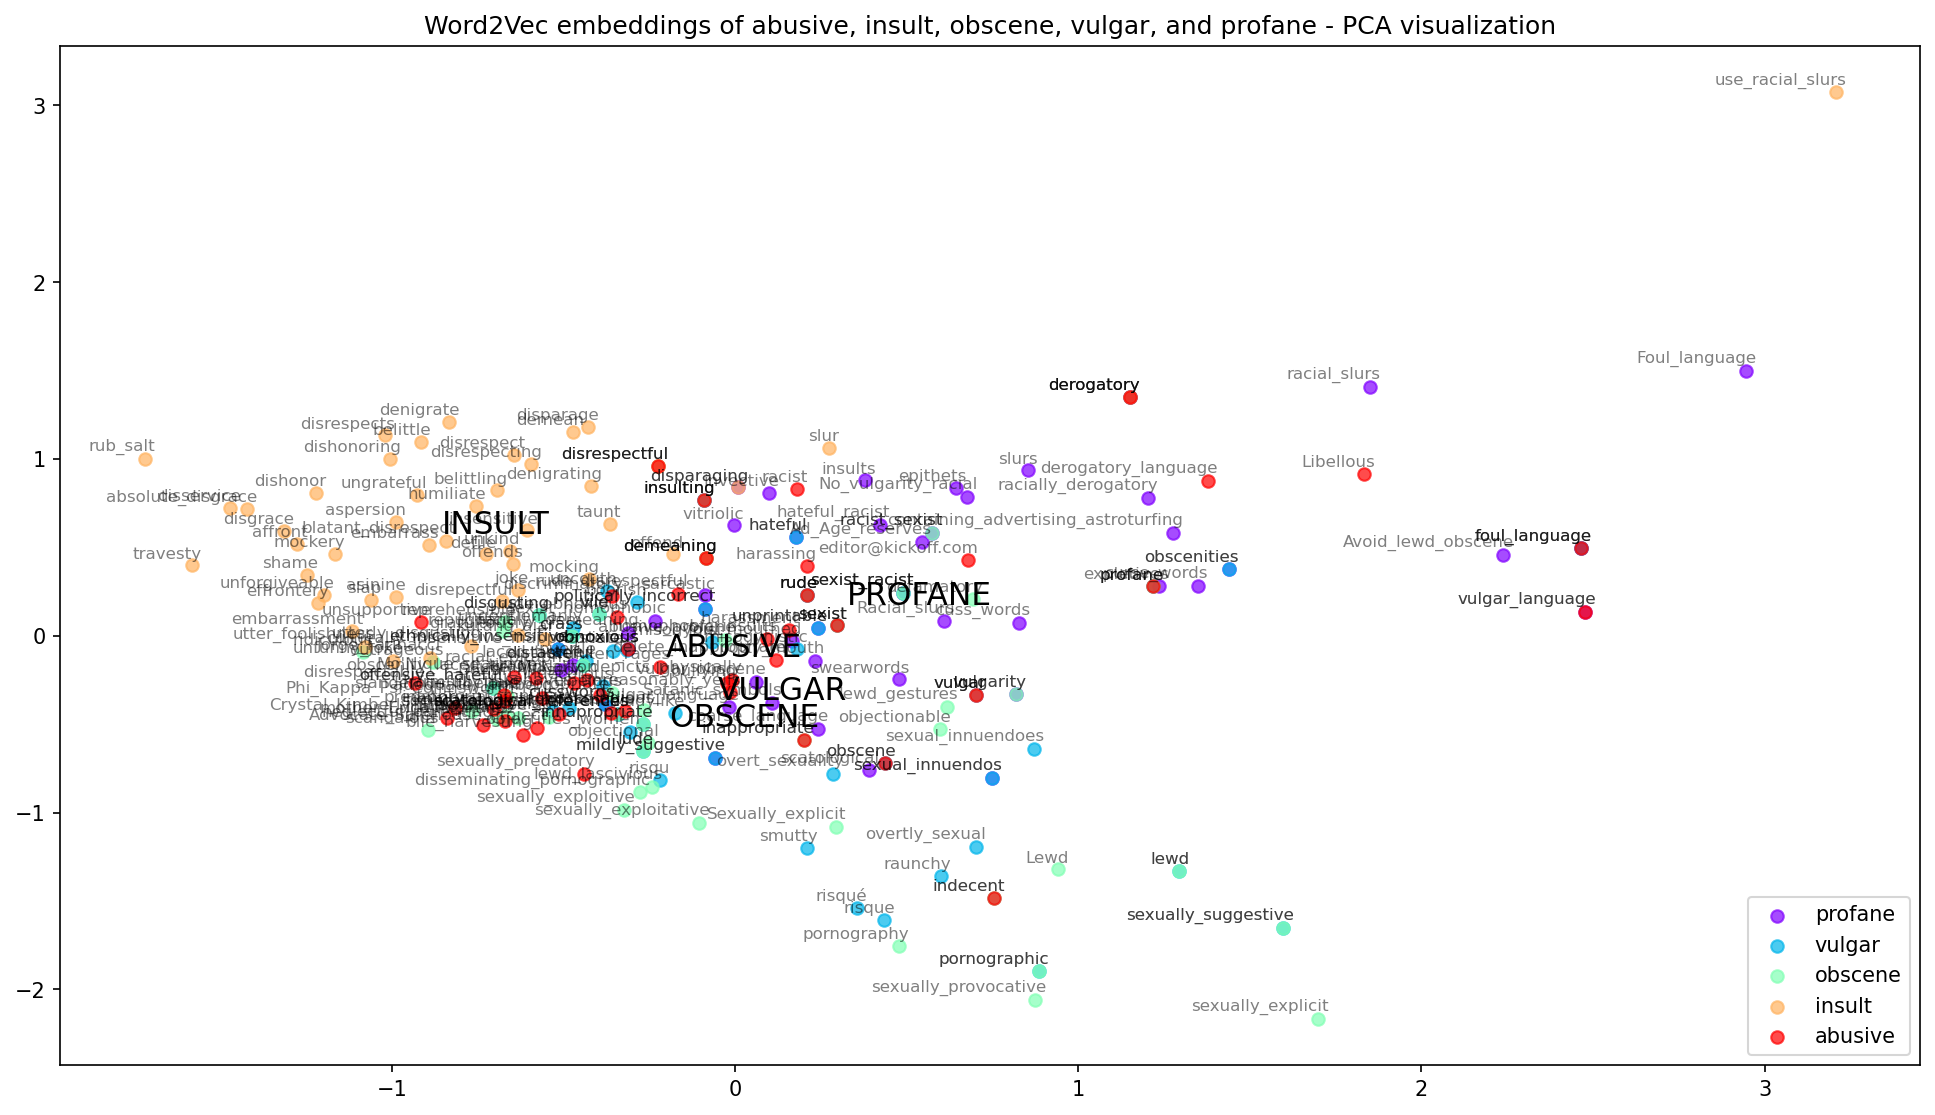
\includegraphics[width=0.33 \linewidth]{Further analysis1 Word2Vec - PCA.png}
%	\caption{\textbf{Further analysis of islands 2, 3 and \textit{abusive} - obscene, insult, discredit, vulgar, profane, and abusive.} Figure shows PCA %visualization of 6 Word2Vec embeddings.}
%	\label{fig:further3}
%\end{figure}

%\begin{figure}[htb]\centering
%	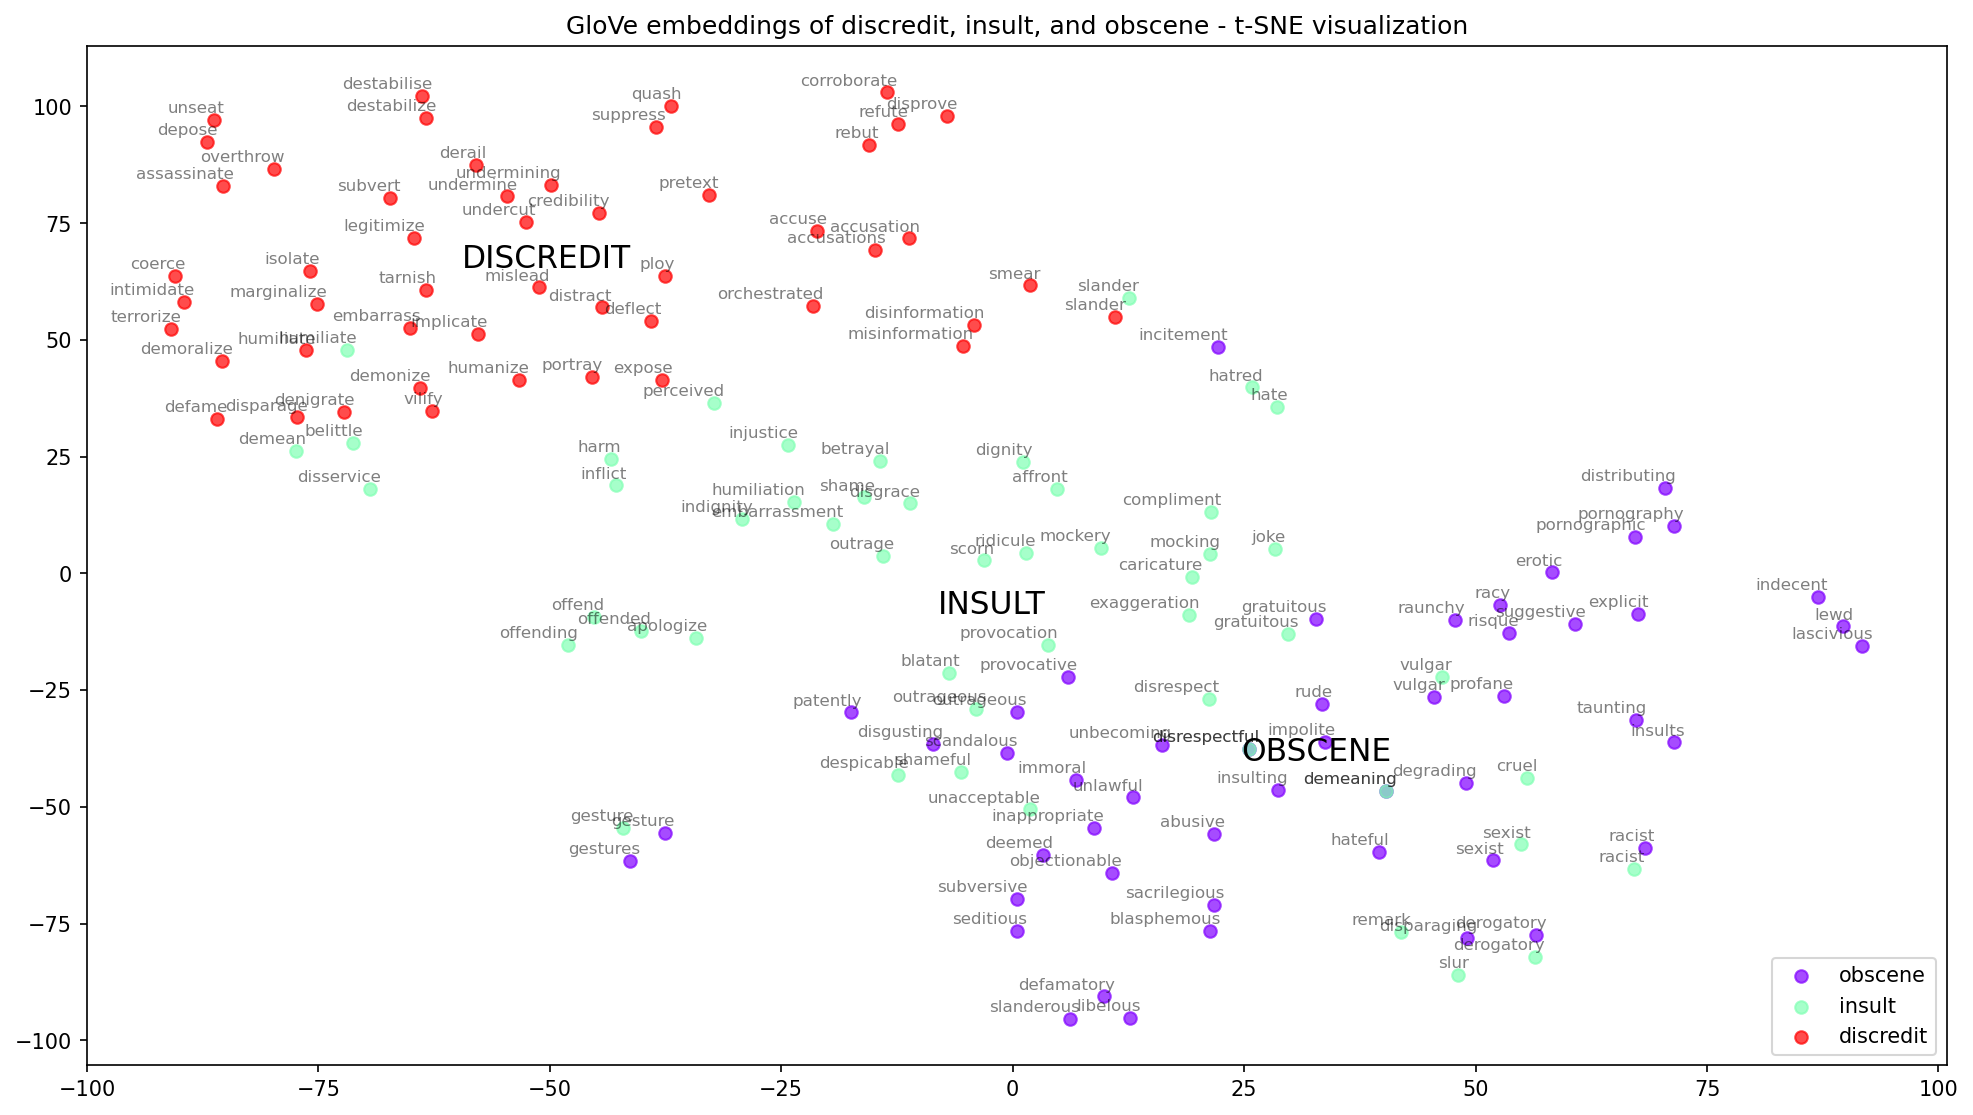
\includegraphics[width=0.33 \linewidth]{Further analysis2 - Glove - t-SNE.png}
%	\caption{\textbf{Further analysis of island 2 - obscene, insult, and discredit.} Figure shows t-SNE visualization of 3 GloVe embeddings.}
%	\label{fig:further2}
%\end{figure}



\section{Discussion}
\label{sec:disc}
Offensive language is known to everybody, as it is very common in the social media. However, we often neglect the fact that is actually a conglomerate of many subgroups, such as sexism, racism, etc. In this paper we wanted to explore offensive language and its structure and we do this by utilizing different natural language processing techniques. 

We used 7 different data sets that contained Twitter and online forum comments. We used traditional techniques, such as TF--IDF, BoW, and LDA and also more advanced approaches such as non-contextual (Word2Vec, GloVe, FastText) and contextual (BERT, keyBERT, USE) embeddings. We found out that each of the approaches provides us with slightly different relations and it is difficult to draw conclusions and we would probably need some help of the linguist professionals. Results also depend on how the comments were obtained and how annotators conceive the meaning of the labels. 

Combining the results from several approaches, we proposed one possible ontology of offensive language.
We inferred there exist 3 groupings that include 4 subgroups of offensive language each. However, even in those groupings there exist subgroups, that are less connected to others. We also found some subgroups that are more separable from others. However, it is important to note that all the subgroups are still tighty connected.

In the future the obtained knowledge could be upgraded with the help of a linguist professional.

%----------------------------------------------------------------------------------------
%	REFERENCE LIST
%----------------------------------------------------------------------------------------
\bibliographystyle{unsrt}
\bibliography{report}


\end{document}